\chapter{Validation of smearing functions}\label{cha:vali}
One might assume that using a Monte Carlo simulation it would be easy to model and emulate the whole process, from collision to detection and reconstruction in the upgraded \abbrLHC. It is possible, but it requires a lot of computing power. Instead one can use one simulation and a mathematical model to calculate the estimated response in the detector. This was validated and used in this thesis to be able to create the data needed for further analysis. 

This was done by using a Monte Carlo simulation of a proton-proton collision and applying the official Truth to reco code, also known as the smearing functions, that was developed using previous studies \citep{ATLAS:LOI2, ATL-PHYS-PUB-2013-004}. to simulate how the detector and the reconstruction is affected by the increased luminosity and the pile-up that comes with this.

The code uses the experimental data from the previous studies to smear the reconstructed energy and momenta, it is from this that the name smearing functions comes.
The key feature of those studies were that the direction of the momenta is unaffected and that only jets and $E^{Miss}_T$ are affected by pile-up. This was confirmed in previous studies and were thus not incorporated into the smearing functions, more in \sectionref{sec:smear}.

\newpage
\section{Smearing functions}\label{sec:smear}
\textbf{Put in introduction? The particles that are directly detectable in \abbrATLAS are:} electron, photon, muon, tau. Aside from this jets can be detected, and from this $E_T^{Miss}$ can be calculated.

This means that the all detectable entities must have their own smearing functions. 

$E_T^{Miss}$, the missing transversal energy, which was discussed in \subsectionref{sec:eo:subsec:mjet}, is calculated by knowing that there should be energy conservation in the collision. In is comprised of different parts, one from neutrinos, one from errors in the other measurements and one from (hopefully) new physics. 

The jet and $E^{Miss}_T$ are the only "parts" which are not unique particles instead they are based either on a shower of particles or the energy which is missing from the conservation of transversal energy. Thus, the pile-up dependence here must simply come from the fact that it is hard to separate the different jets and that with several different collisions occurring makes it hard to accurately measure the total energy.

The electron and photon have the same smearing since they are both detected in a similar way.  Perhaps add more to the introduction about each part of the detector. or simply write that here?

The muon is special since it is detected in the muon spectrometer.  

Tau is detected similarly to electron and photon.

These smearing functions are designed so that they take into account the efficiency of the different detectors, limitations as well as their dependence on pile-up. They also take into account how all this varies depending on the measured entries energy or momenta.

The terminology is that data before smearing, simulated data, is denoted as data at a truth level or truth data. Data after smearing, which is comparable to what is measured, reconstructed or reco data as discussed in \subsectionref{sec:eo:subsec:reco}.
\newpage
\section{Validation}\label{sec:vali}
To validate the smearing functions a comparison with \citep{ATL-PHYS-PUB-2013-004} was made where the standard deviation, depending on the energy of momentum value of an entity, was given, see \sectionref{cha:vali:sec:expr}. To calculate this some simulated processes were needed to extract data, see \tableref{tab:backproc}. 
\begin{SCtable}[][ht]
\begin{tabular}{|l|l|}
\hline
Data & Process \\ \hline
Electron & W$\rightarrow e\nu$ \\
Muon & W$\rightarrow \mu \nu$ \\
Tau & W$\rightarrow \tau \nu$ \\
$\gamma$ & $\gamma$ + Jet sample \\
Jets & Jet sample \\
$E_T^{Miss}$ & Z$\rightarrow \nu \nu$ + Jet sample \\ \hline
\end{tabular}
\caption{Different processes from where data has been taken. Each sample is a simulation of a physical process, the simulation names can be found in \appendixref{cha:datasets}}
\label{tab:backproc}
\end{SCtable}

By plotting the data for each data point before and after the smearing function, for that data point had been used, one can verify the functions. This is done looking at the reco data for a given truth energy or momentum value. Since the smearing functions take a lot of things into account the match will not be a fine line, see \figureref{fig:tau:2}.

By fitting a Gaussian curve to this data will then result in the mean value, and the standard deviation. The mean value is not of interest for the purposes of the thesis, though the standard deviation is since it is this which is used in the validation. The standard deviation is equivalent to \abbrRMS (Root mean square) and is also known as the resolution of the data. It will from here on be denoted \abbrRMS or $\sigma$.

This resolution is then compared to previous results, \citep{ATL-PHYS-PUB-2013-004}, and finally confirmed or demented.

To get enough and thorough statistics enough data must be available for a given truth energy or momenta and the analysis must be specific enough to only look at a minute interval around this point.
\newpage
\section{Results}\label{cha:vali:sec:results}
As discussed above, the method was to plot the data against its smeared counterpart and through this determine the \abbrRMS, ($\sigma$) to see if it conforms to the expected values.

Since there are only slightly differences depending on pile-up these are not shown except for $E_T^{Miss}$ and jets. Also only one energy value is shown for simplicity, though the comparison was done for different energy values.

Pile-up is fixed at 60 is nothing else is said used simply as a benchmark.

The images are, as the comparison, often divided depending on the different $\eta$ values.

All results are summarized in \tableref{tab:RMSval}. 
\newpage
\subsection{Electron and photon}
Since these interact very  similarly in the detector, their smearing functions are identical.
The slice value represents at which value of unsmeared energy or momentum this smearing occurs. 
%\begin{figure}[!htbp]
%  \centering 
%  \subfloat[eleta1. \label{fig:elph:1}]{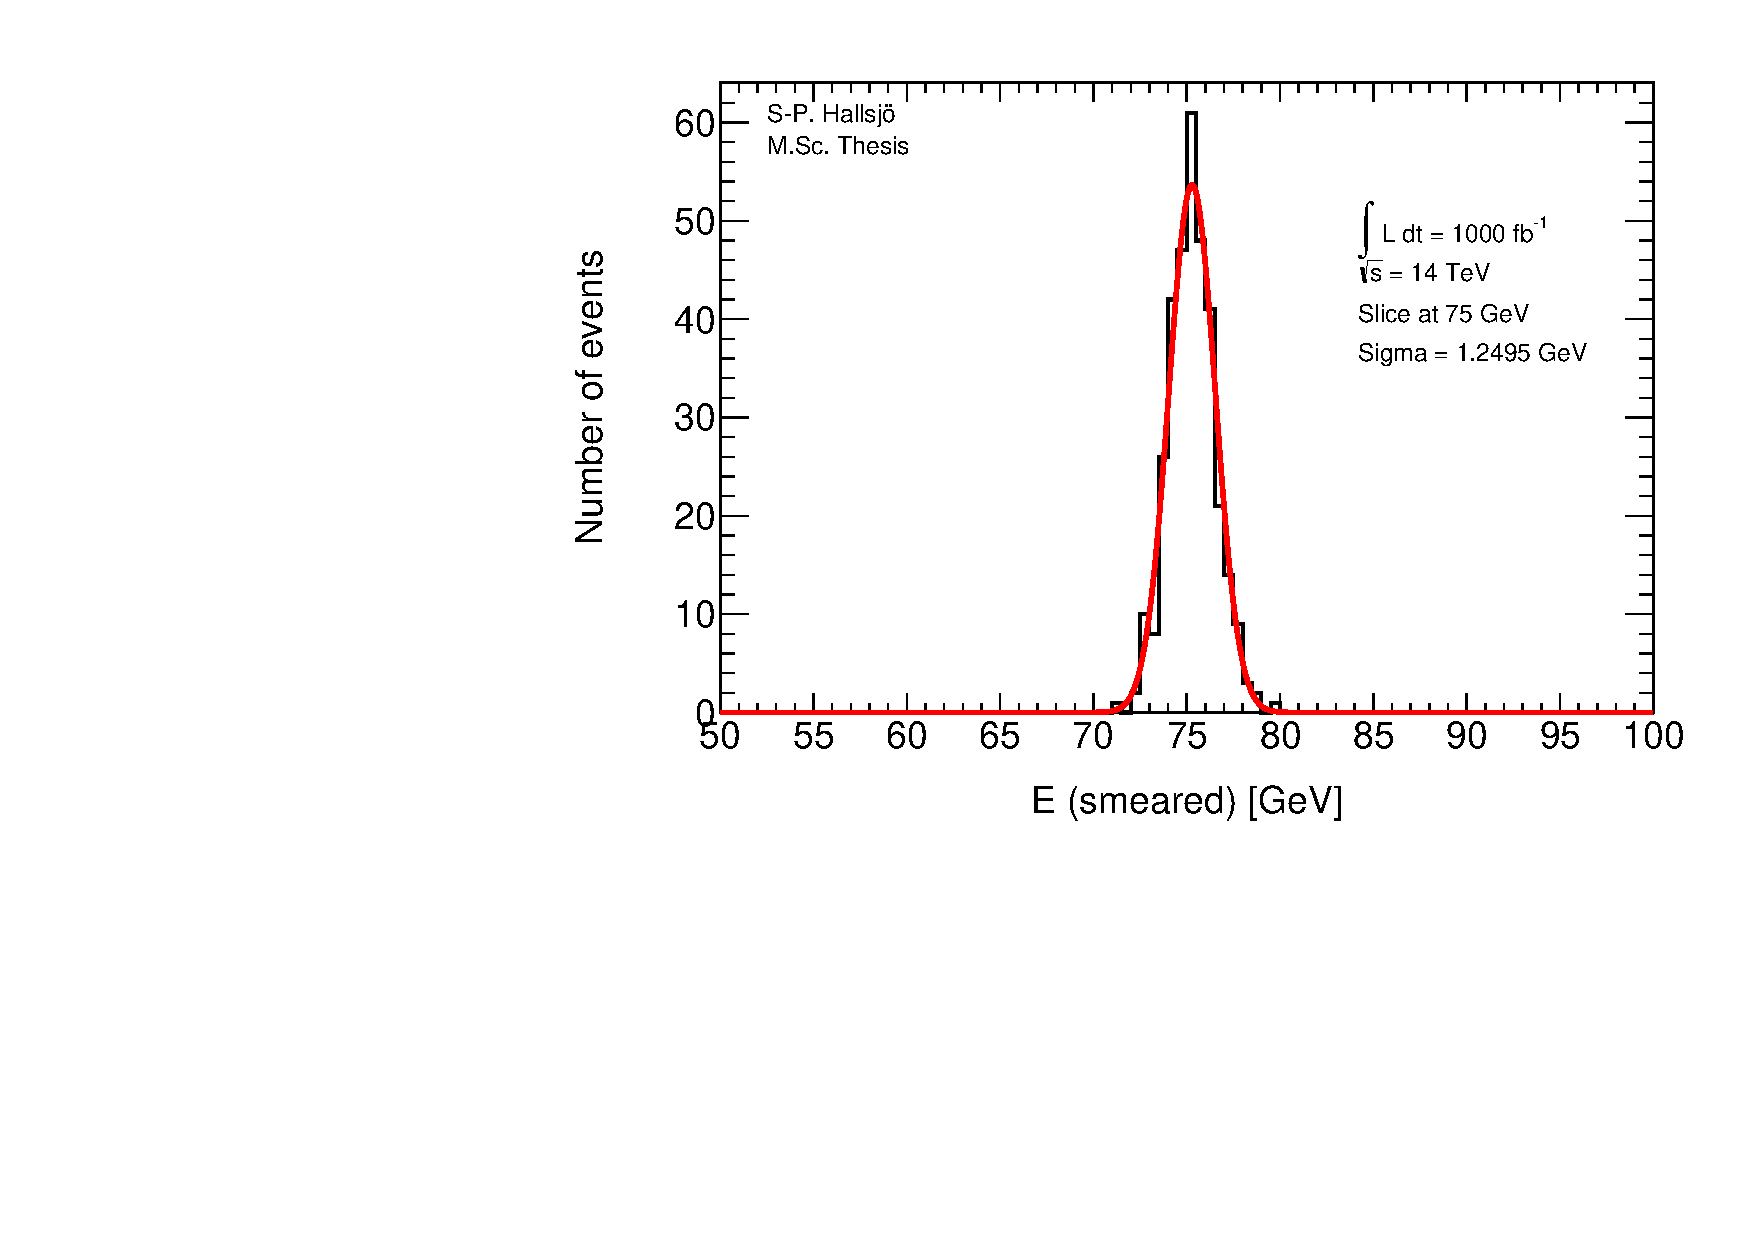
\includegraphics[width=0.5\textwidth]{eleta1.pdf}}% 
%\hfill
%  \subfloat[eleta2.\label{fig:elph:2}]{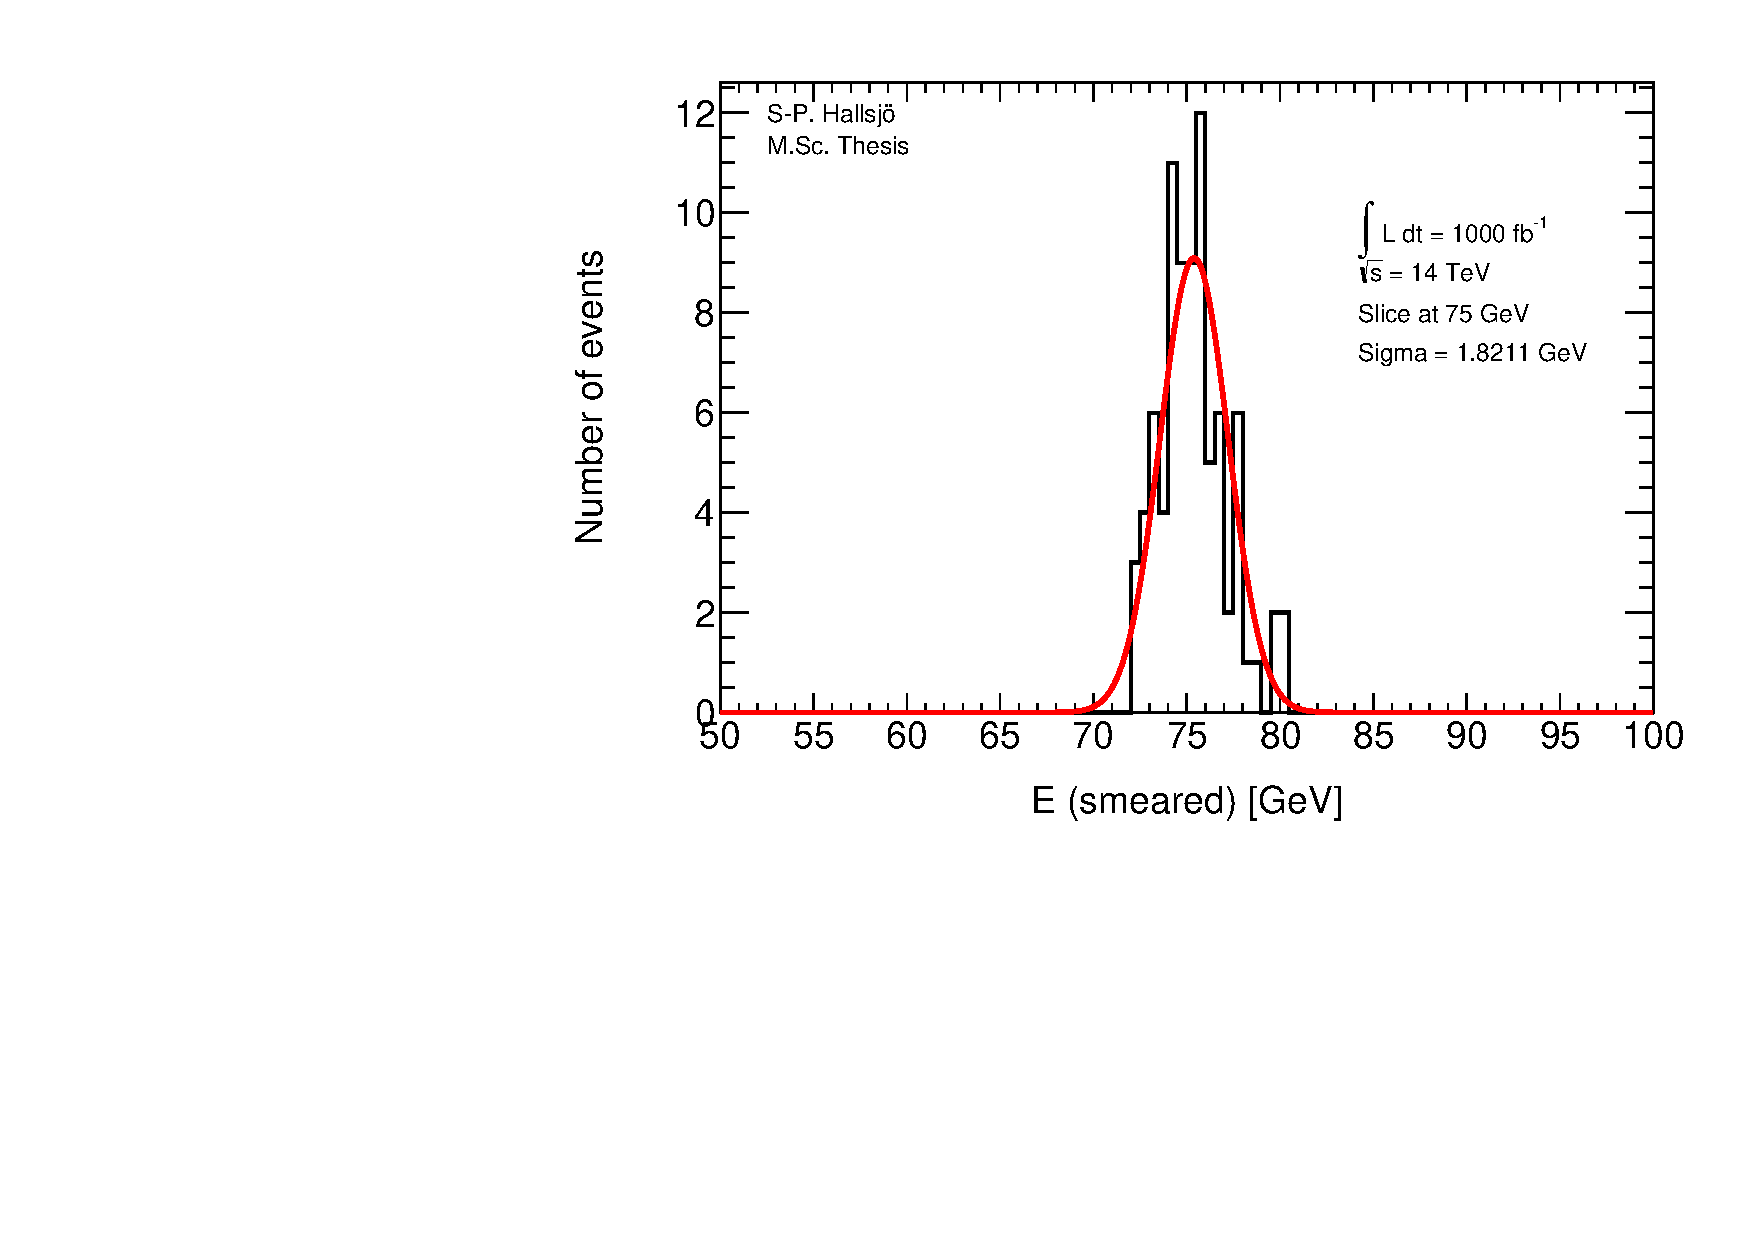
\includegraphics[width=0.5\textwidth]{eleta2.pdf}} 
%  \caption{el and ph eta}
%  \label{fig:elph}
%\end{figure}

%\begin{figure}[!htbp]
%% If it needs to be split.
%  \ContinuedFloat 
%  \centering 
%  \subfloat[pheta1. \label{fig:elph:3}]{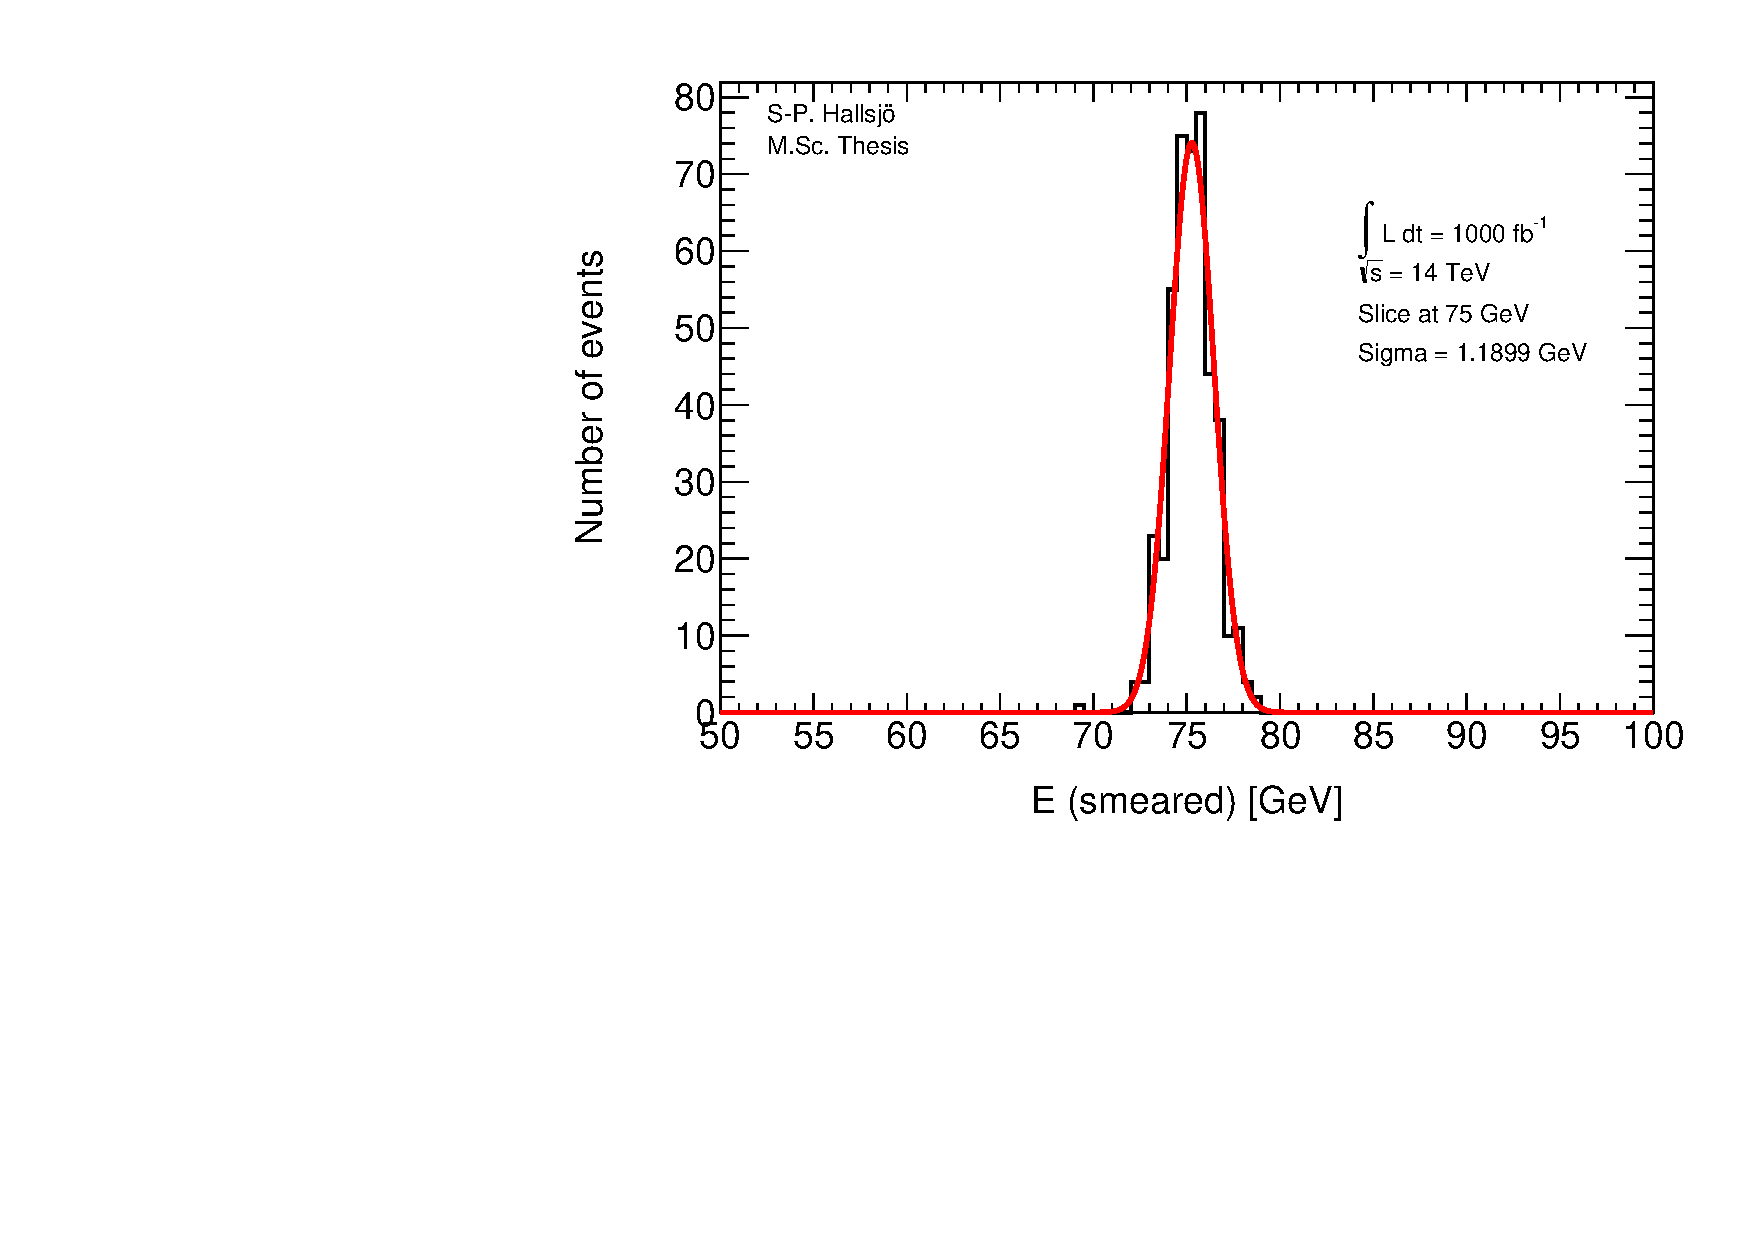
\includegraphics[width=0.5\textwidth]{pheta1.pdf}}% 
%  \hfill
%  \subfloat[pheta2.\label{fig:elph:4}]{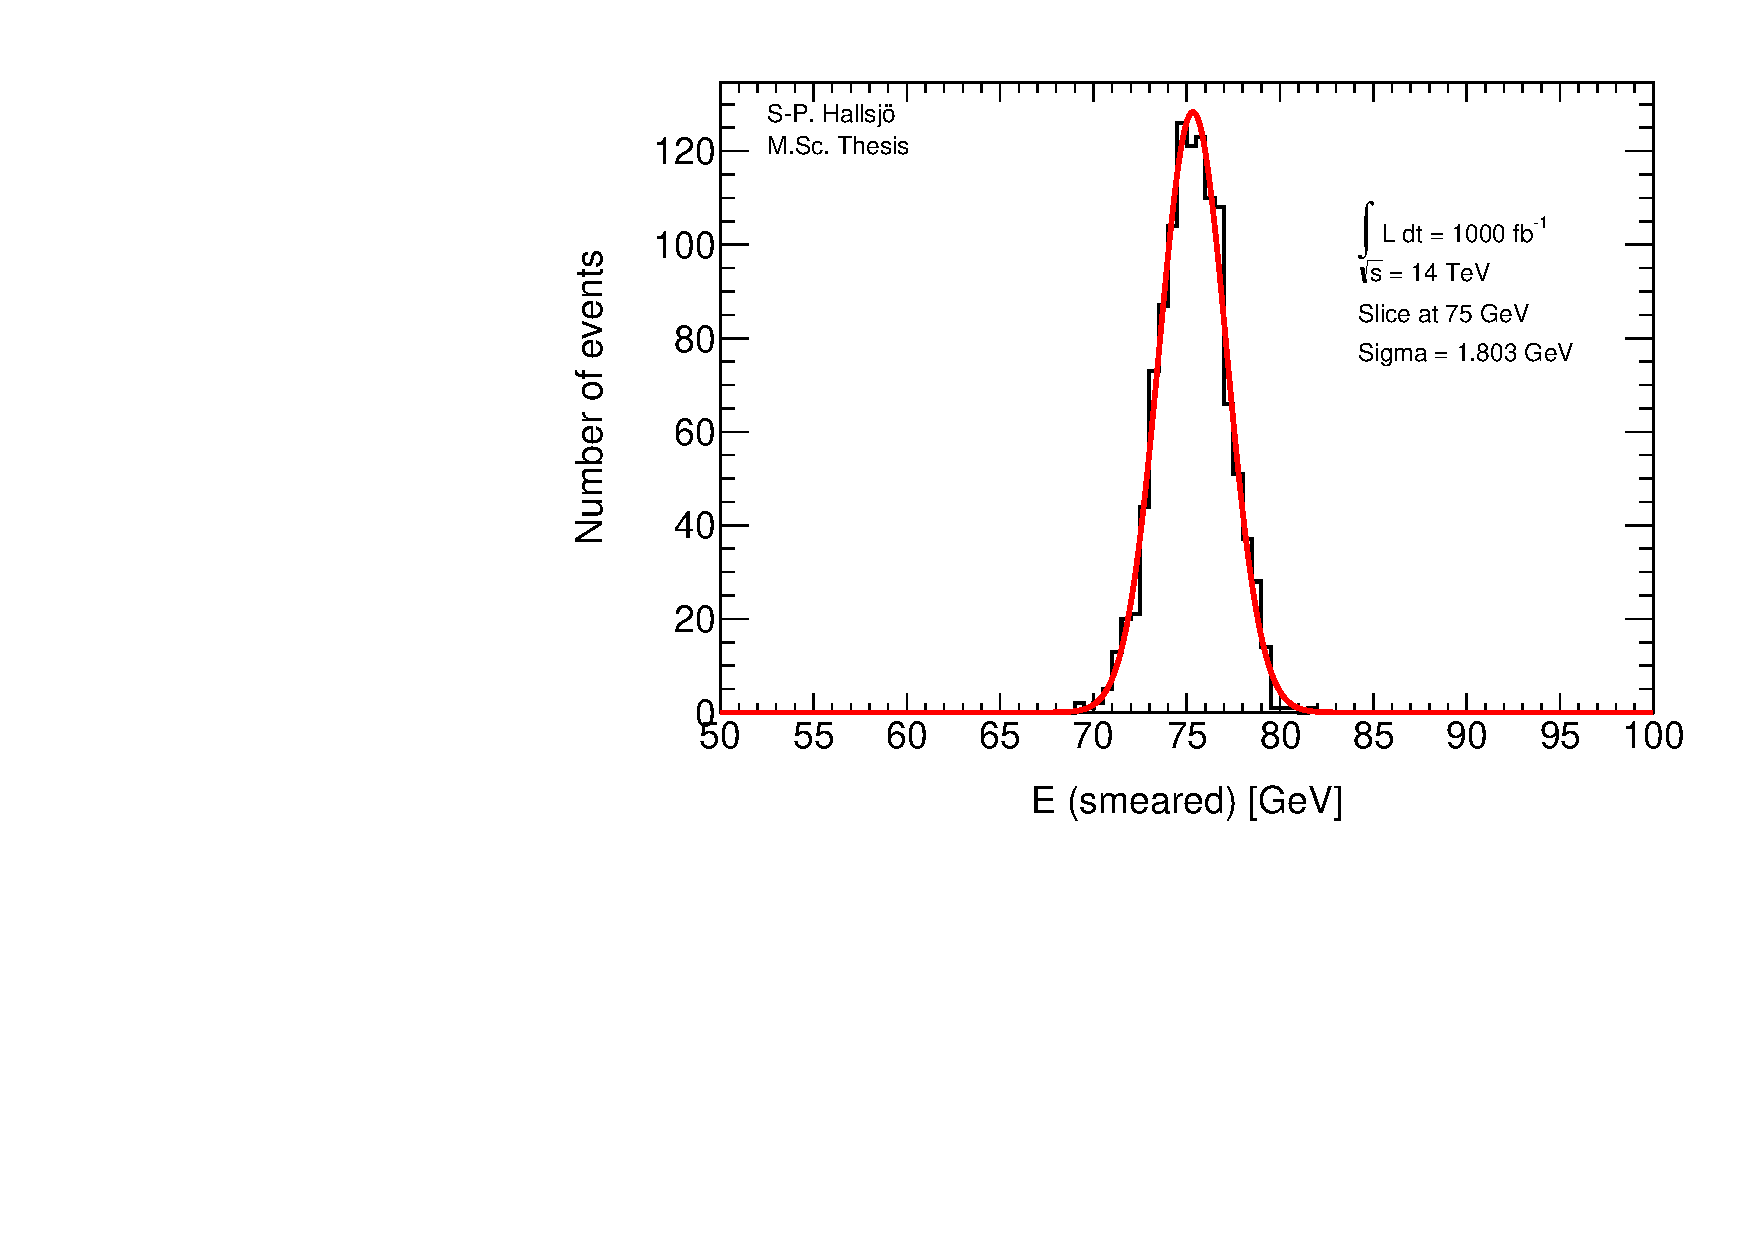
\includegraphics[width=0.5\textwidth]{pheta2.pdf}} 
%  \setcounter{figure}{1}
%  \caption[]{el and ph eta}
%  \label{fig:elph}
%\end{figure} 
%\setcounter{figure}{1}

 \begin{figure}[H] %!ht
    \subfloat[Electron smearing for $\abs{\eta}<1.4$. \label{fig:elph:1}]{%
    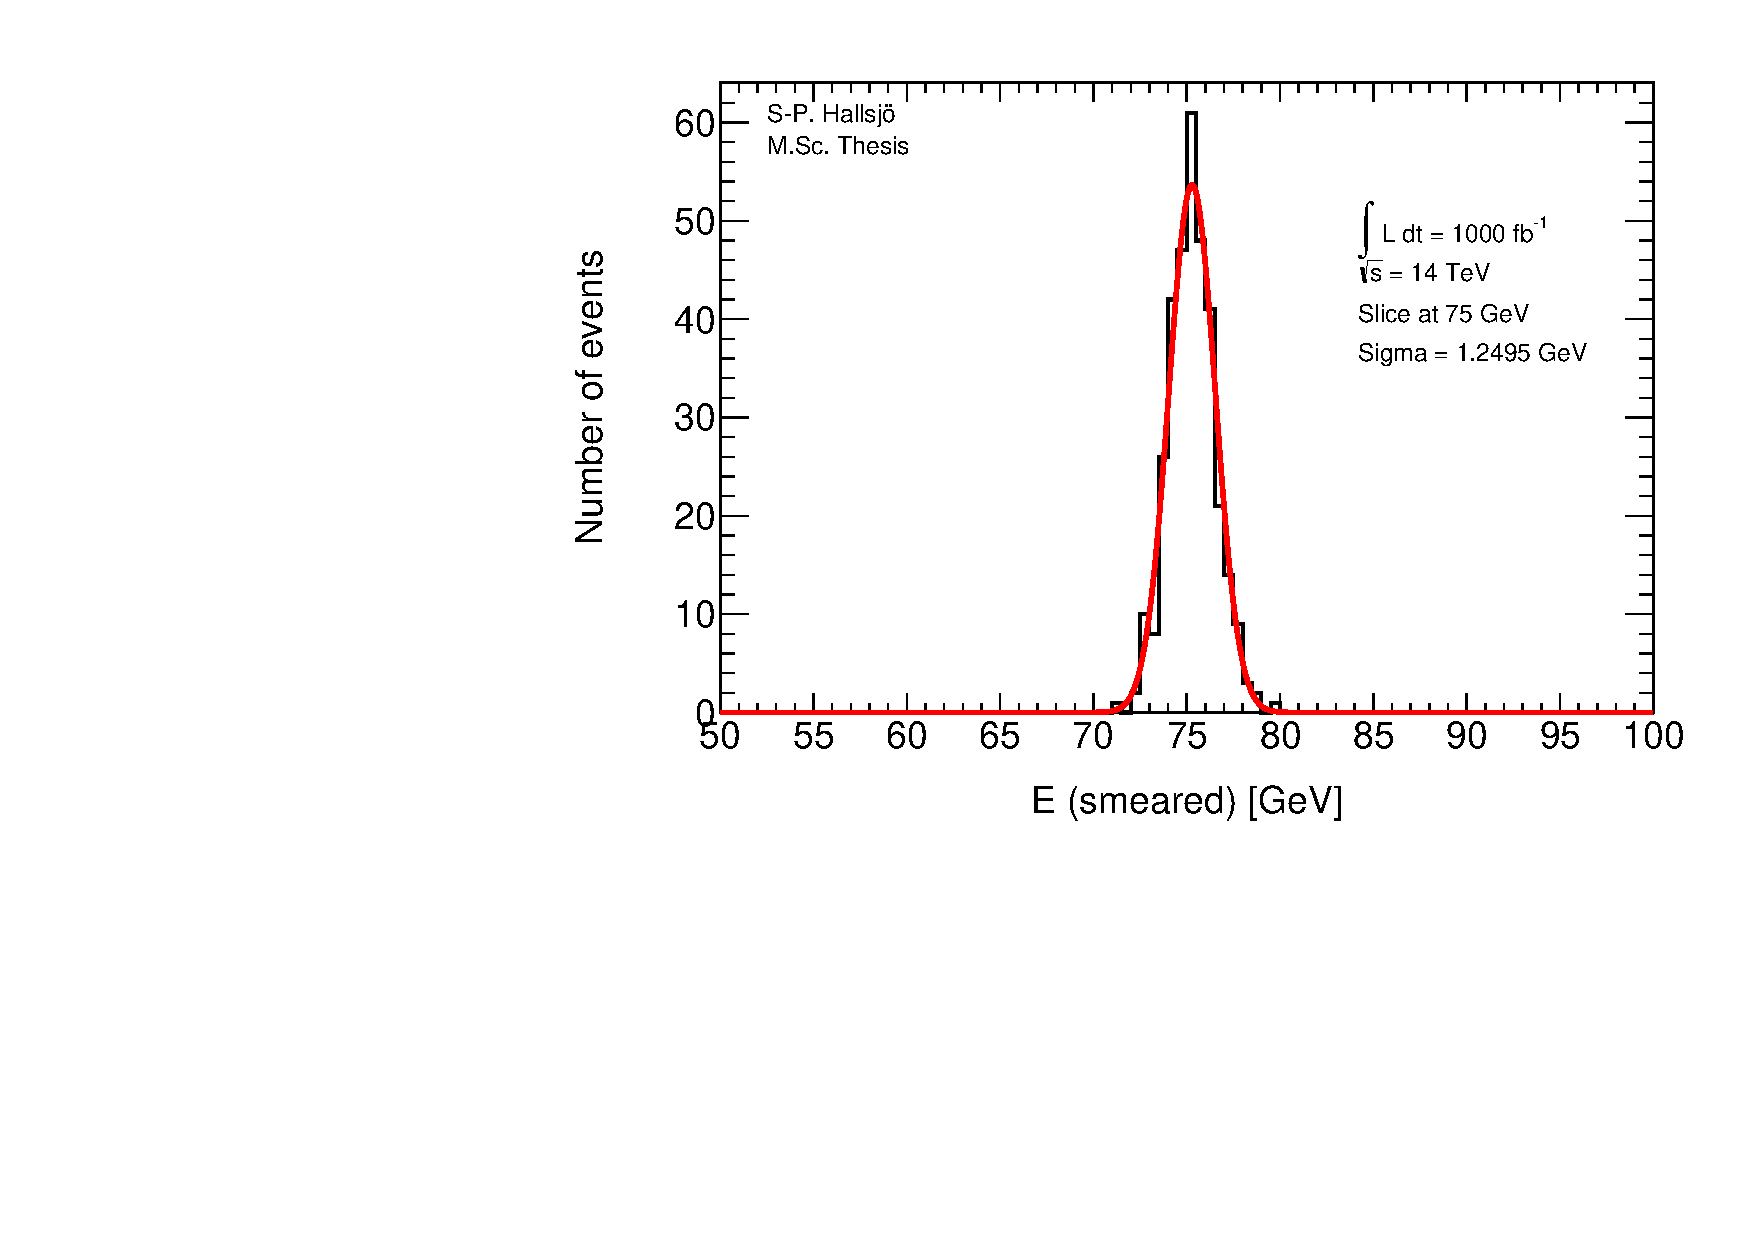
\includegraphics[width=0.5\textwidth]{eleta1.pdf}
    }
    \hfill
\subfloat[Electron smearing for $1.4<\abs{\eta}<2.47$.\label{fig:elph:2}]{%
      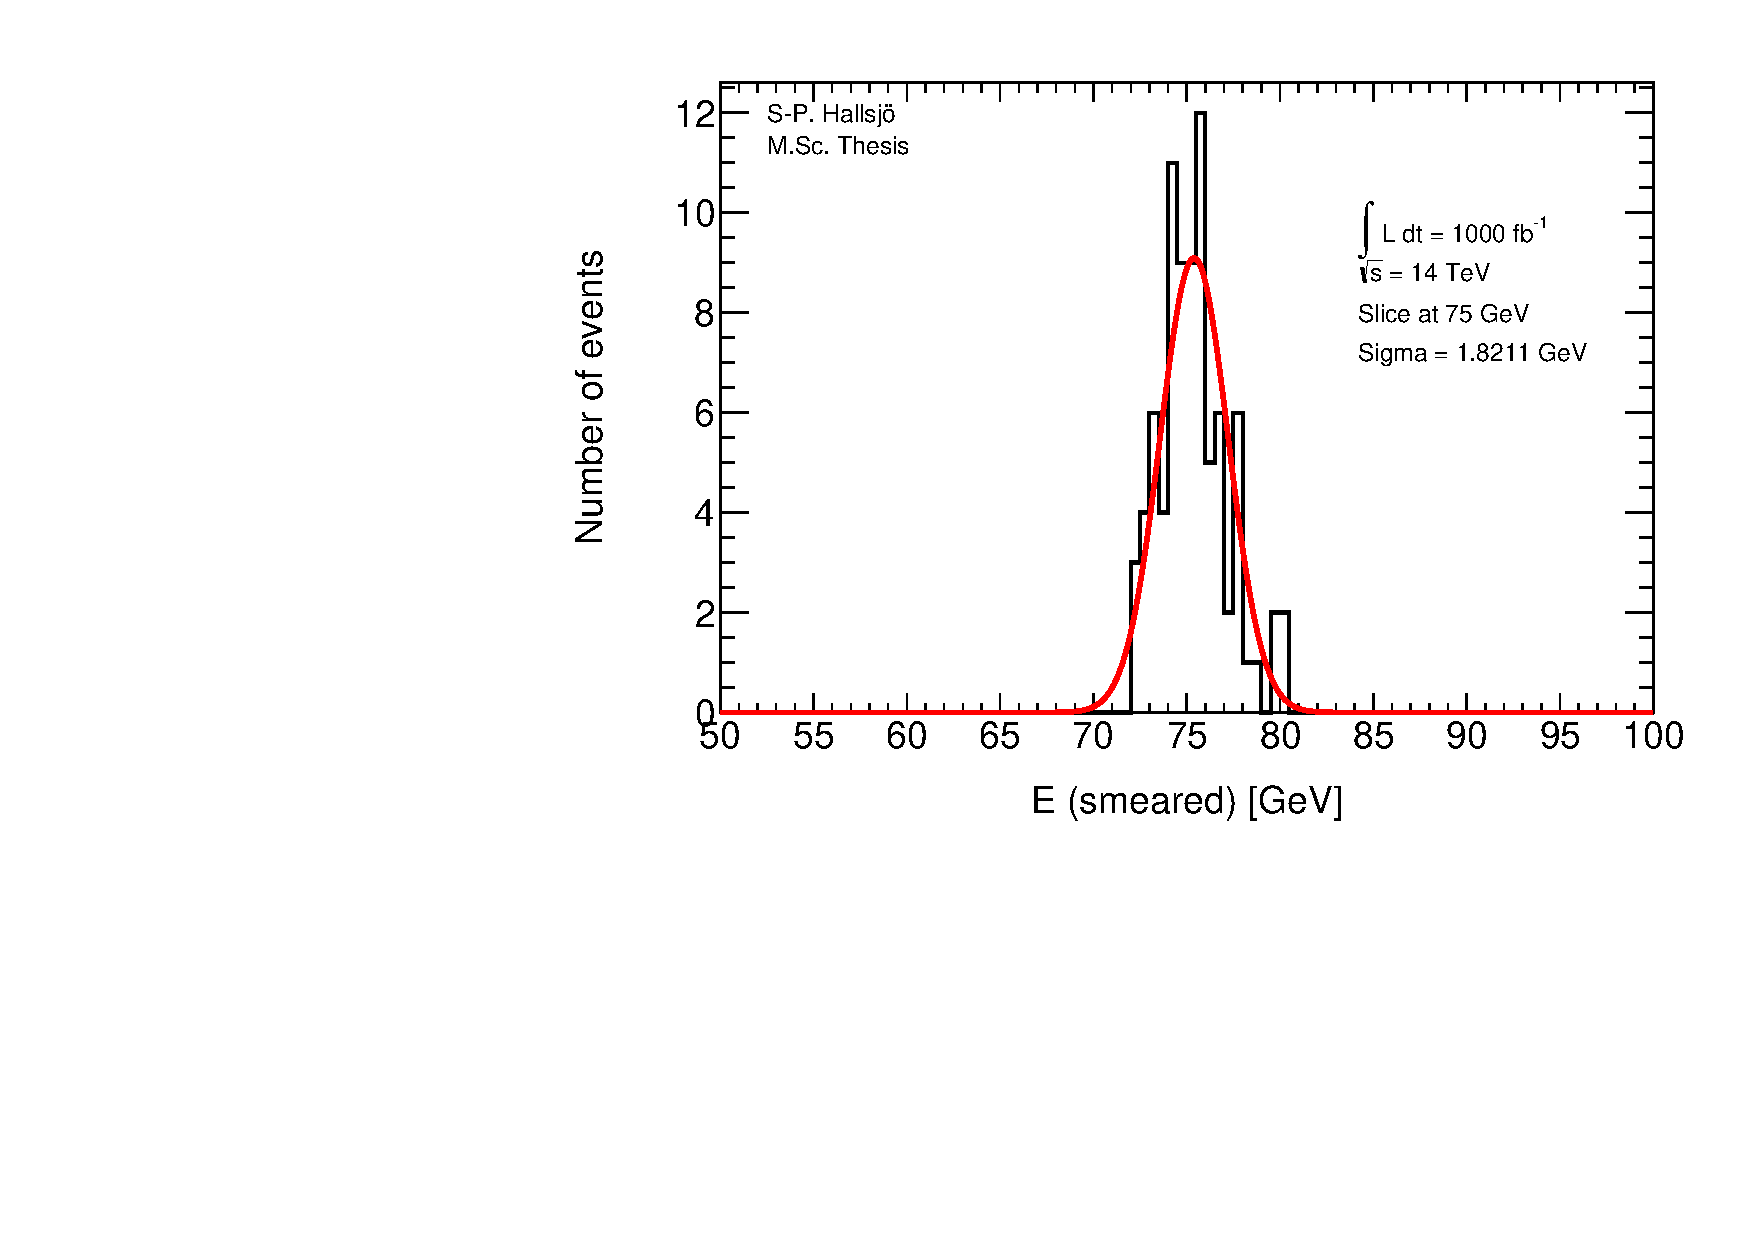
\includegraphics[width=0.5\textwidth]{eleta2.pdf}
    }
    \hfill
        \subfloat[Photon smearing for $\abs{\eta}<1.4$. \label{fig:elph:3}]{%
     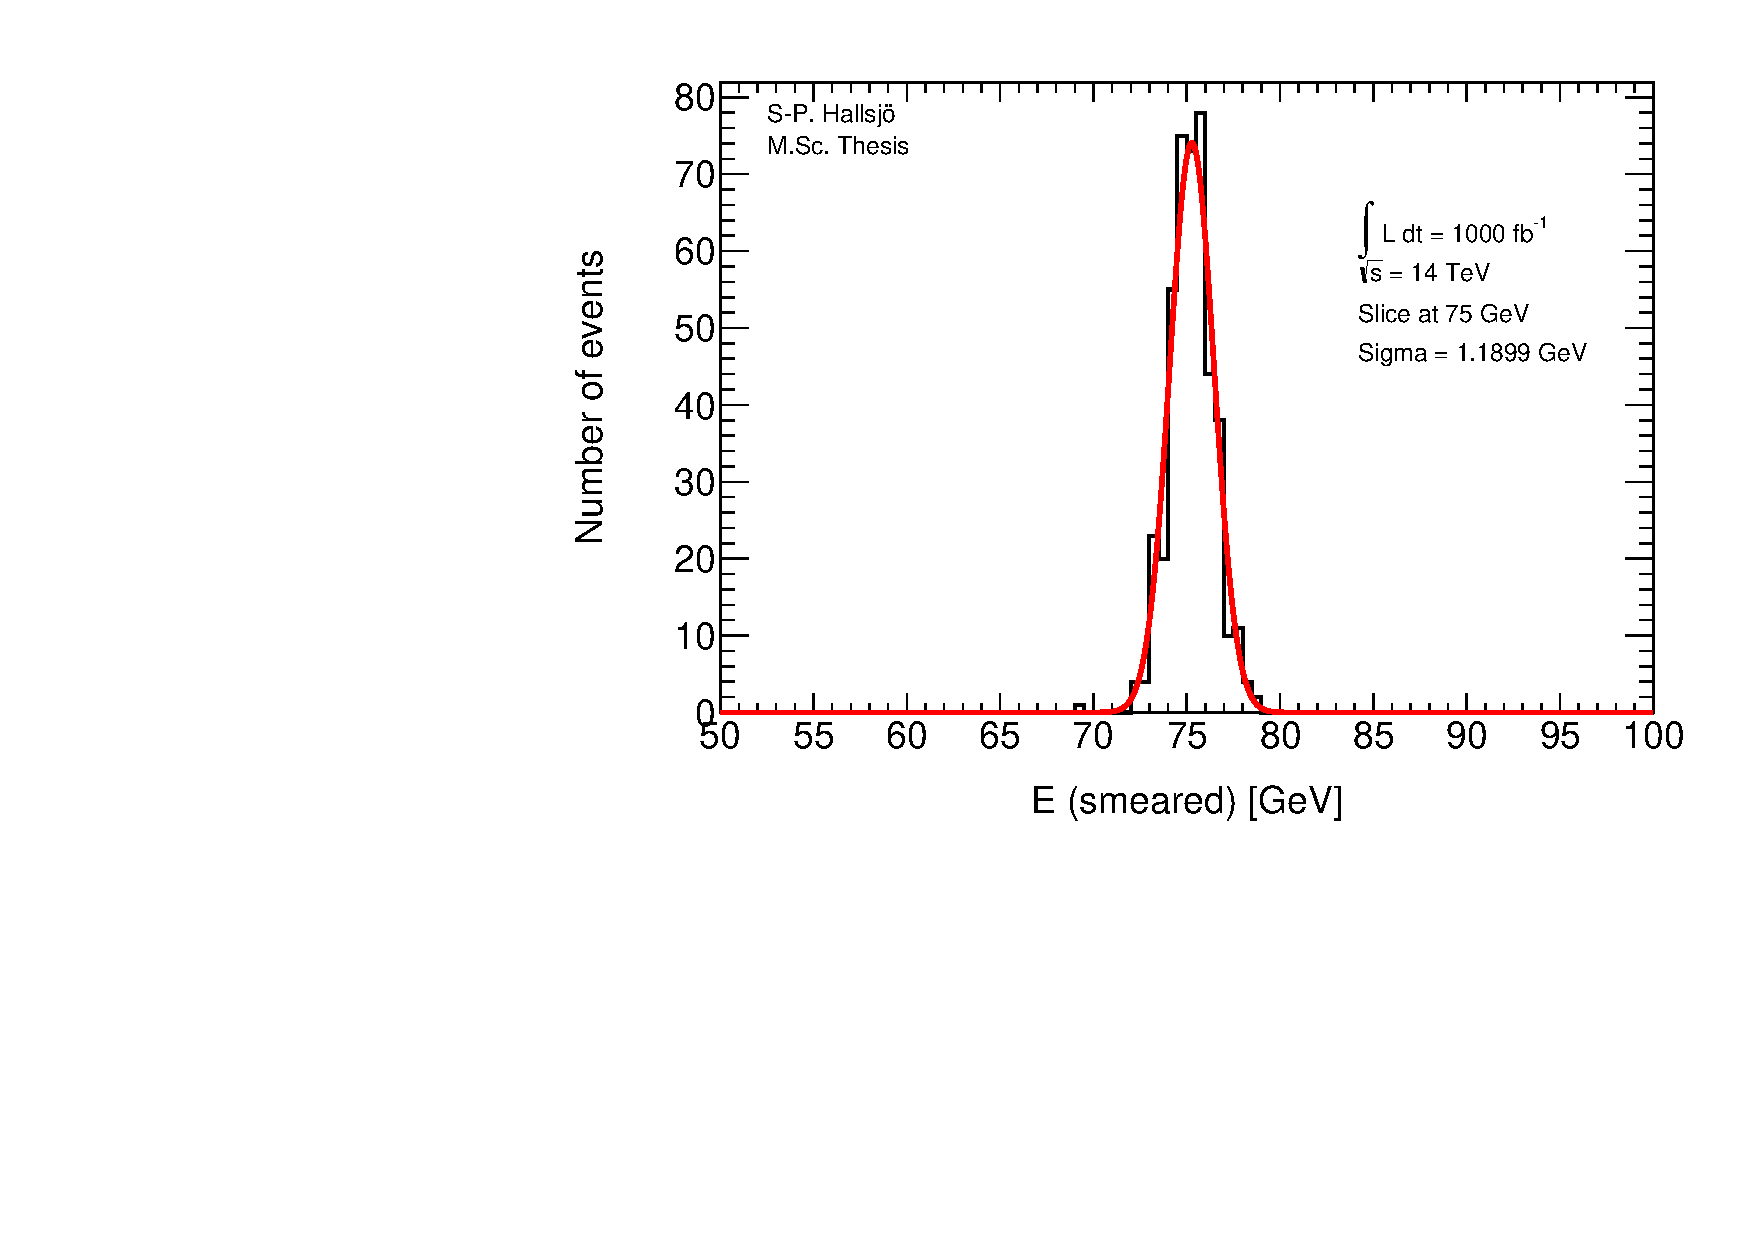
\includegraphics[width=0.5\textwidth]{pheta1.pdf}
    }
    \hfill
\subfloat[Photon smearing for $1.4<\abs{\eta}<2.47$.\label{fig:elph:4}]{%
     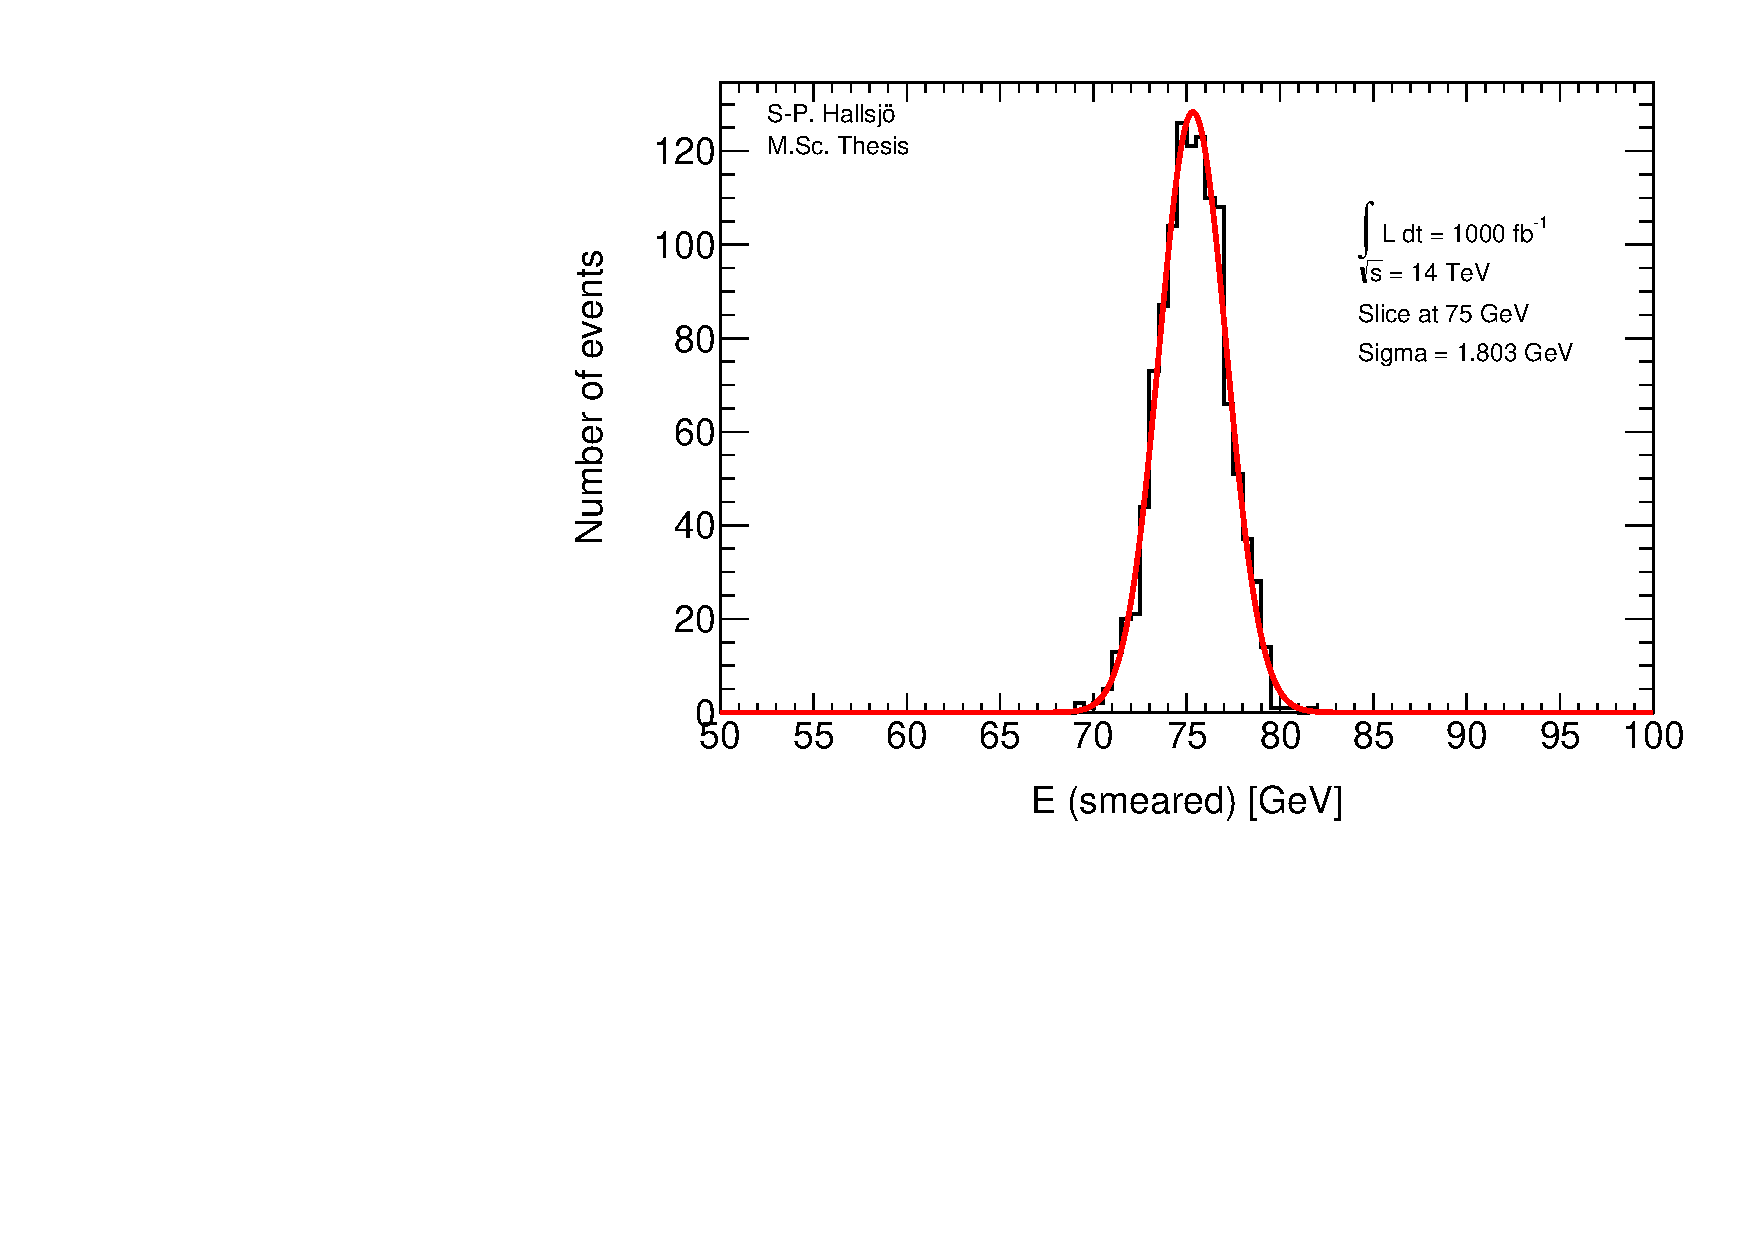
\includegraphics[width=0.5\textwidth]{pheta2.pdf}
    }
    \caption{Photon and electron smearing plots.}
    \label{fig:elph}
\end{figure}
\newpage
\subsection{Muon}
 \begin{figure}[H] %!ht
    \subfloat[Muon smearing for $\abs{\eta}<1.05$. \label{fig:muon:1}]{%
     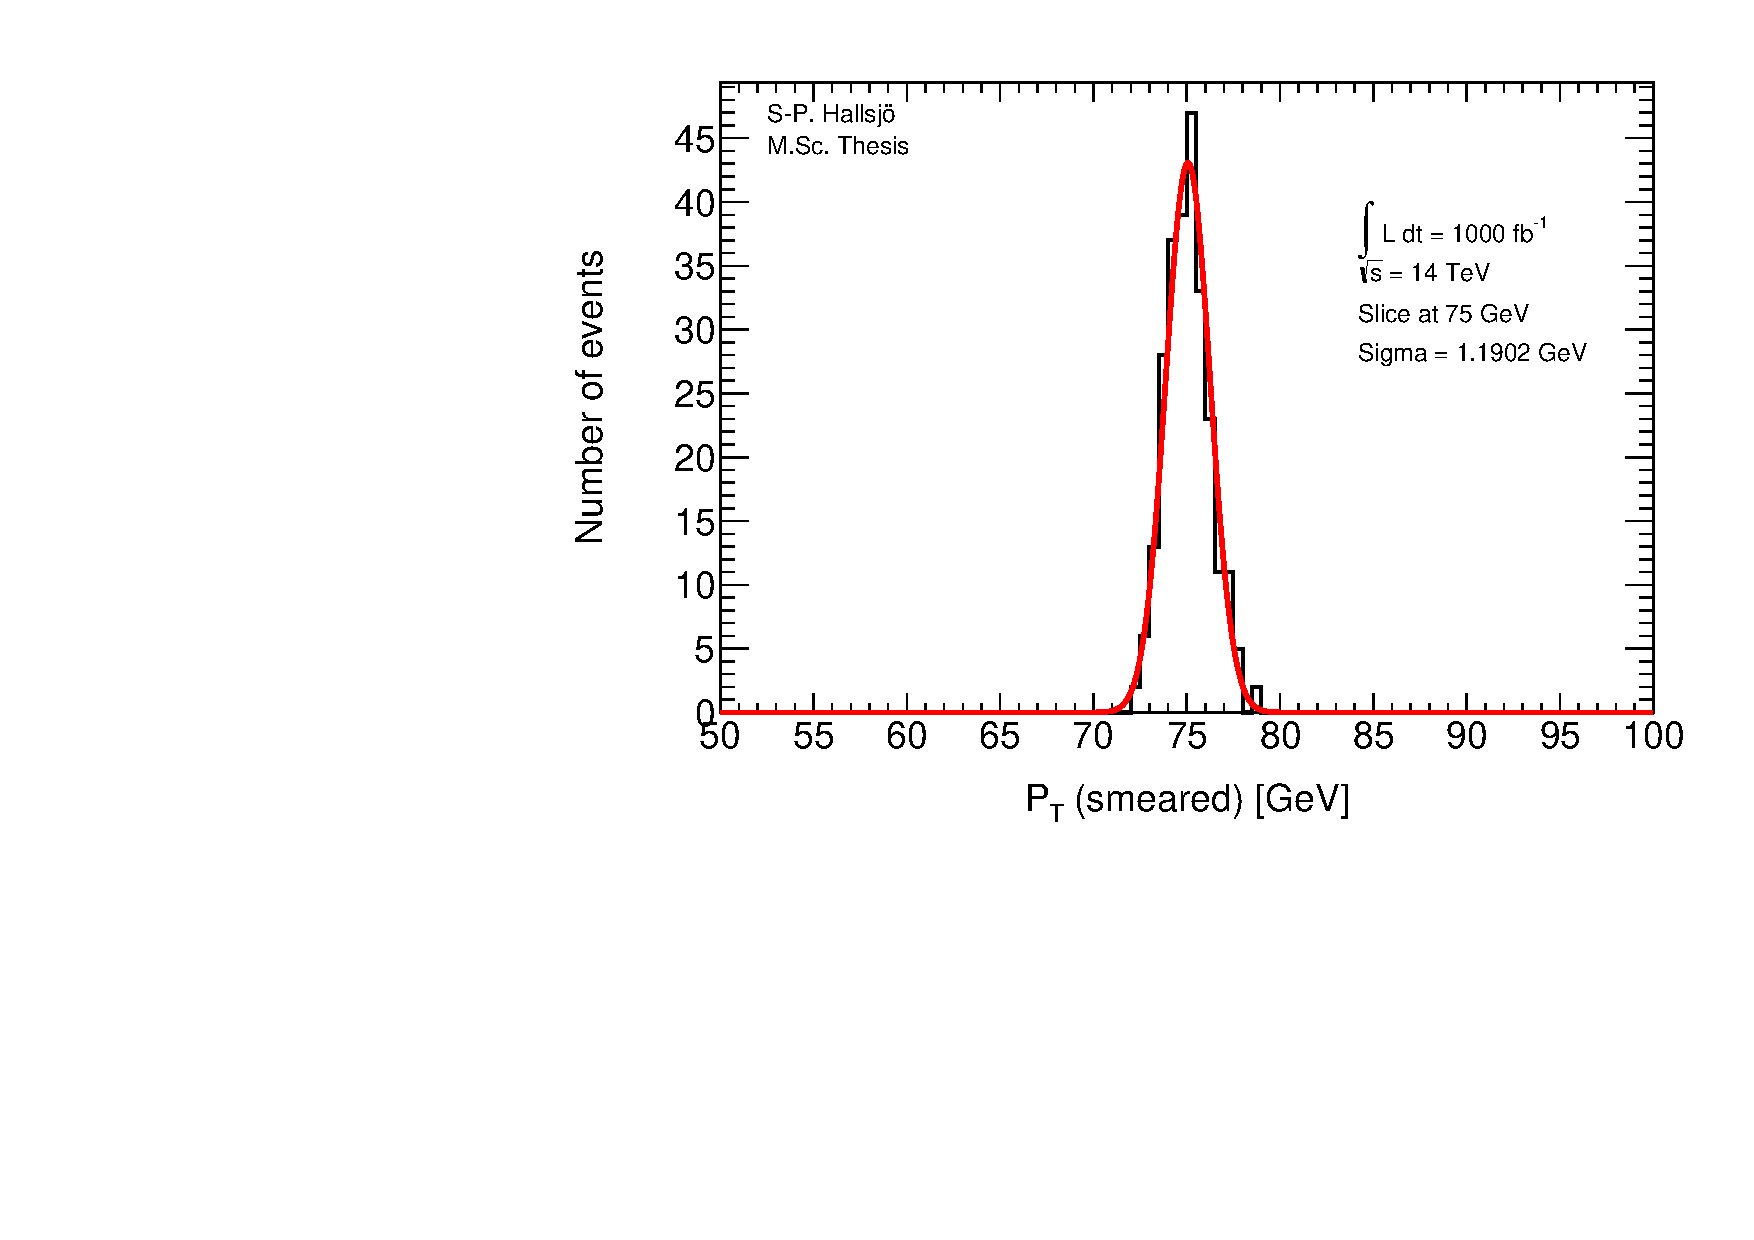
\includegraphics[width=0.5\textwidth]{mueta1.pdf}
    }
    \hfill
    \subfloat[Muon smearing for $1.05<\abs{\eta}$.\label{fig:muon:2}]{%
      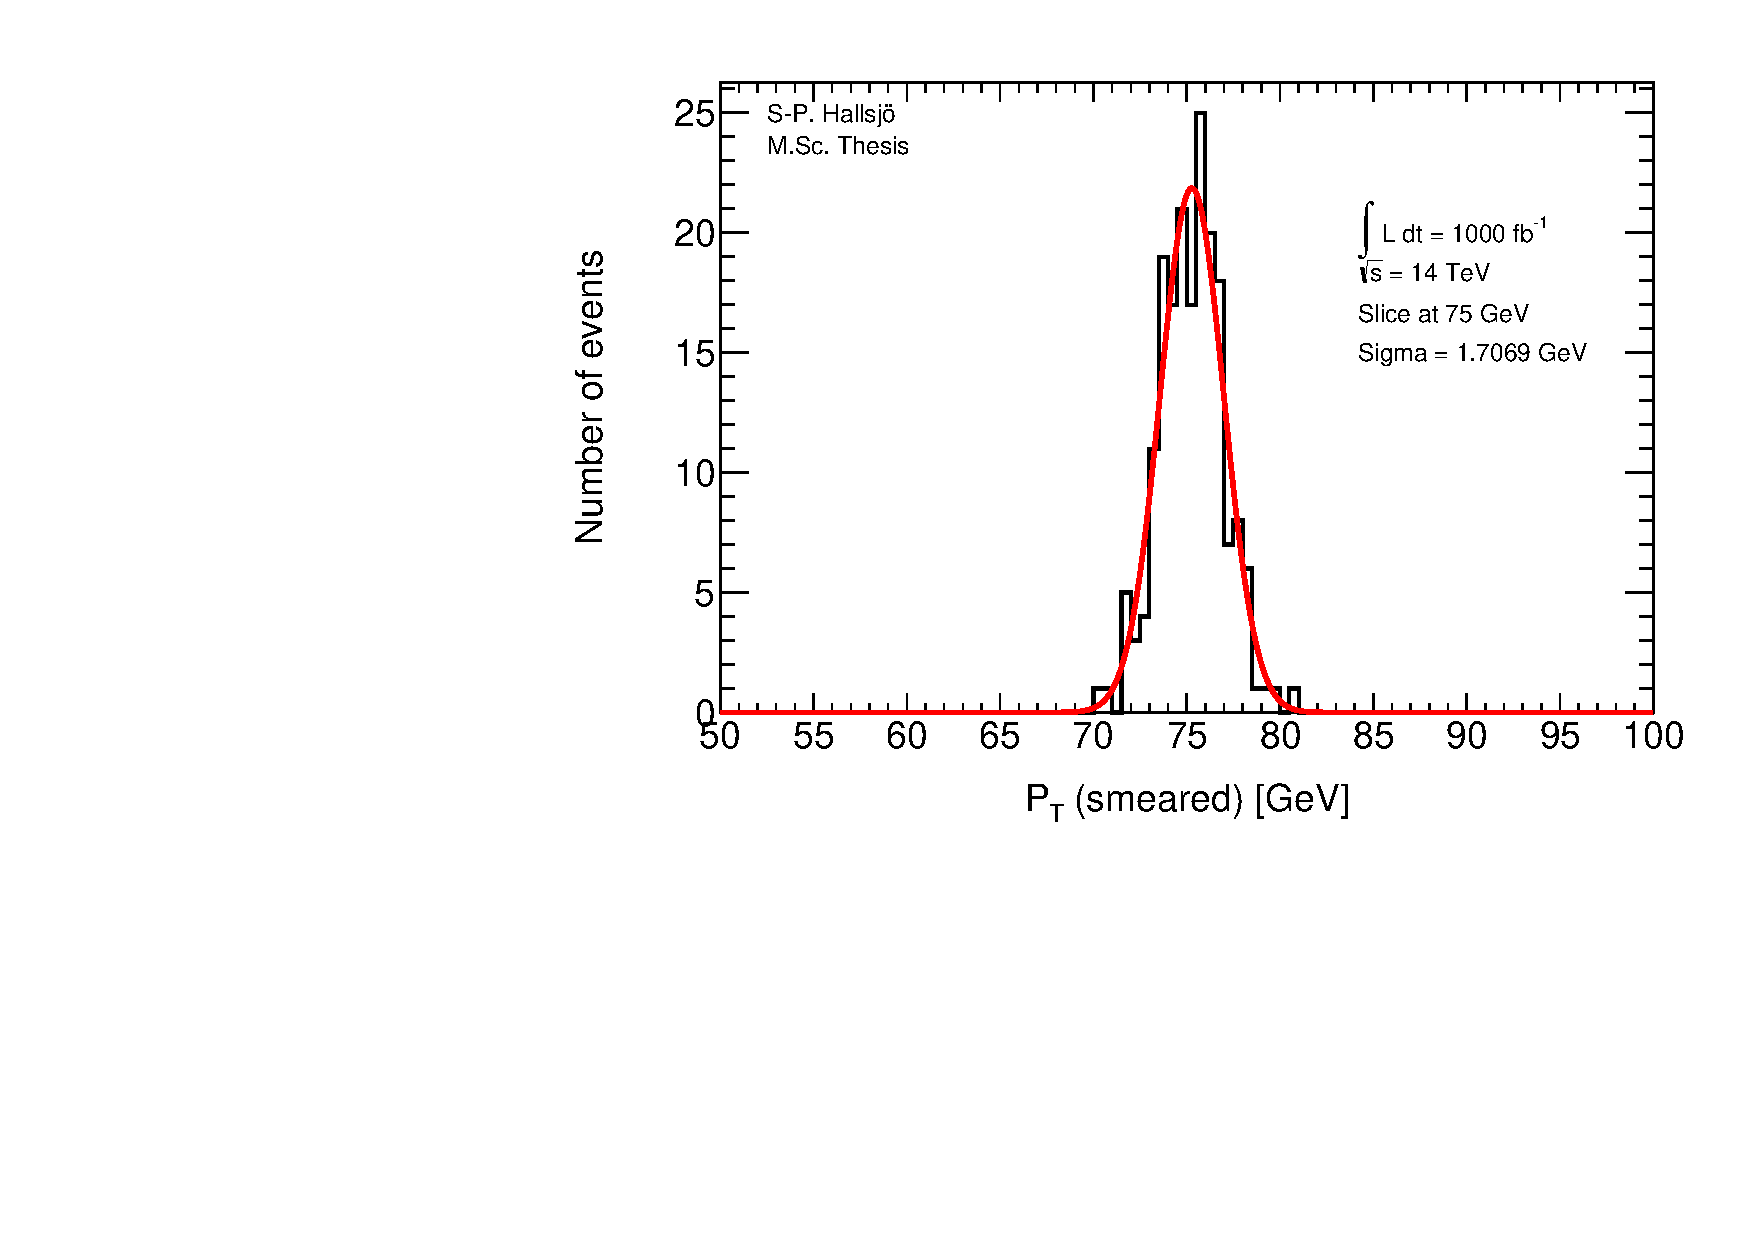
\includegraphics[width=0.5\textwidth]{mueta2.pdf}
    }
    \caption{Muon smearing plots.}
    \label{fig:muon}
  \end{figure}
\subsection{Tau}
 \begin{figure}[H] %!ht
    \subfloat[Tau smearing. \label{fig:tau:1}]{%
     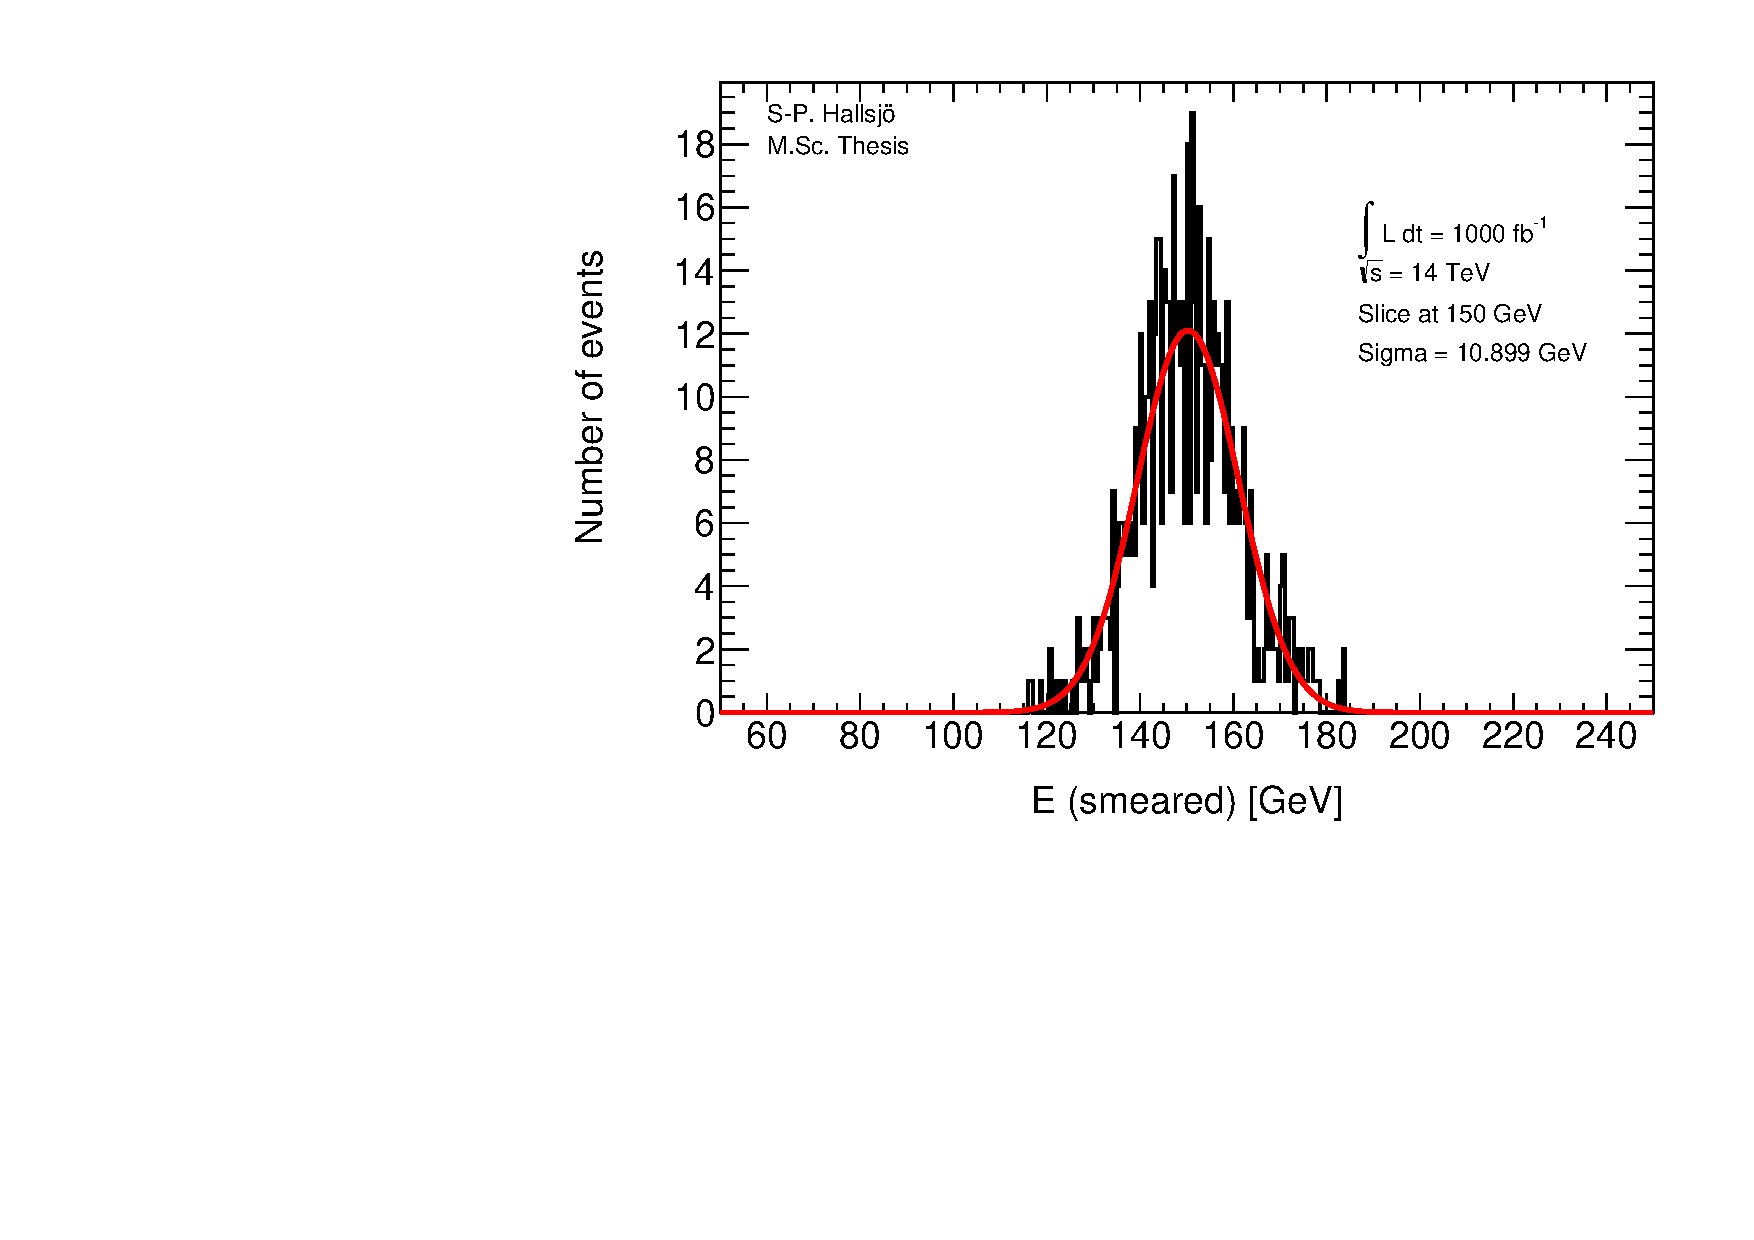
\includegraphics[width=0.5\textwidth]{tau.pdf}
    }
    \hfill
    \subfloat[Tau energy vs smeared. \label{fig:tau:2}]{%
      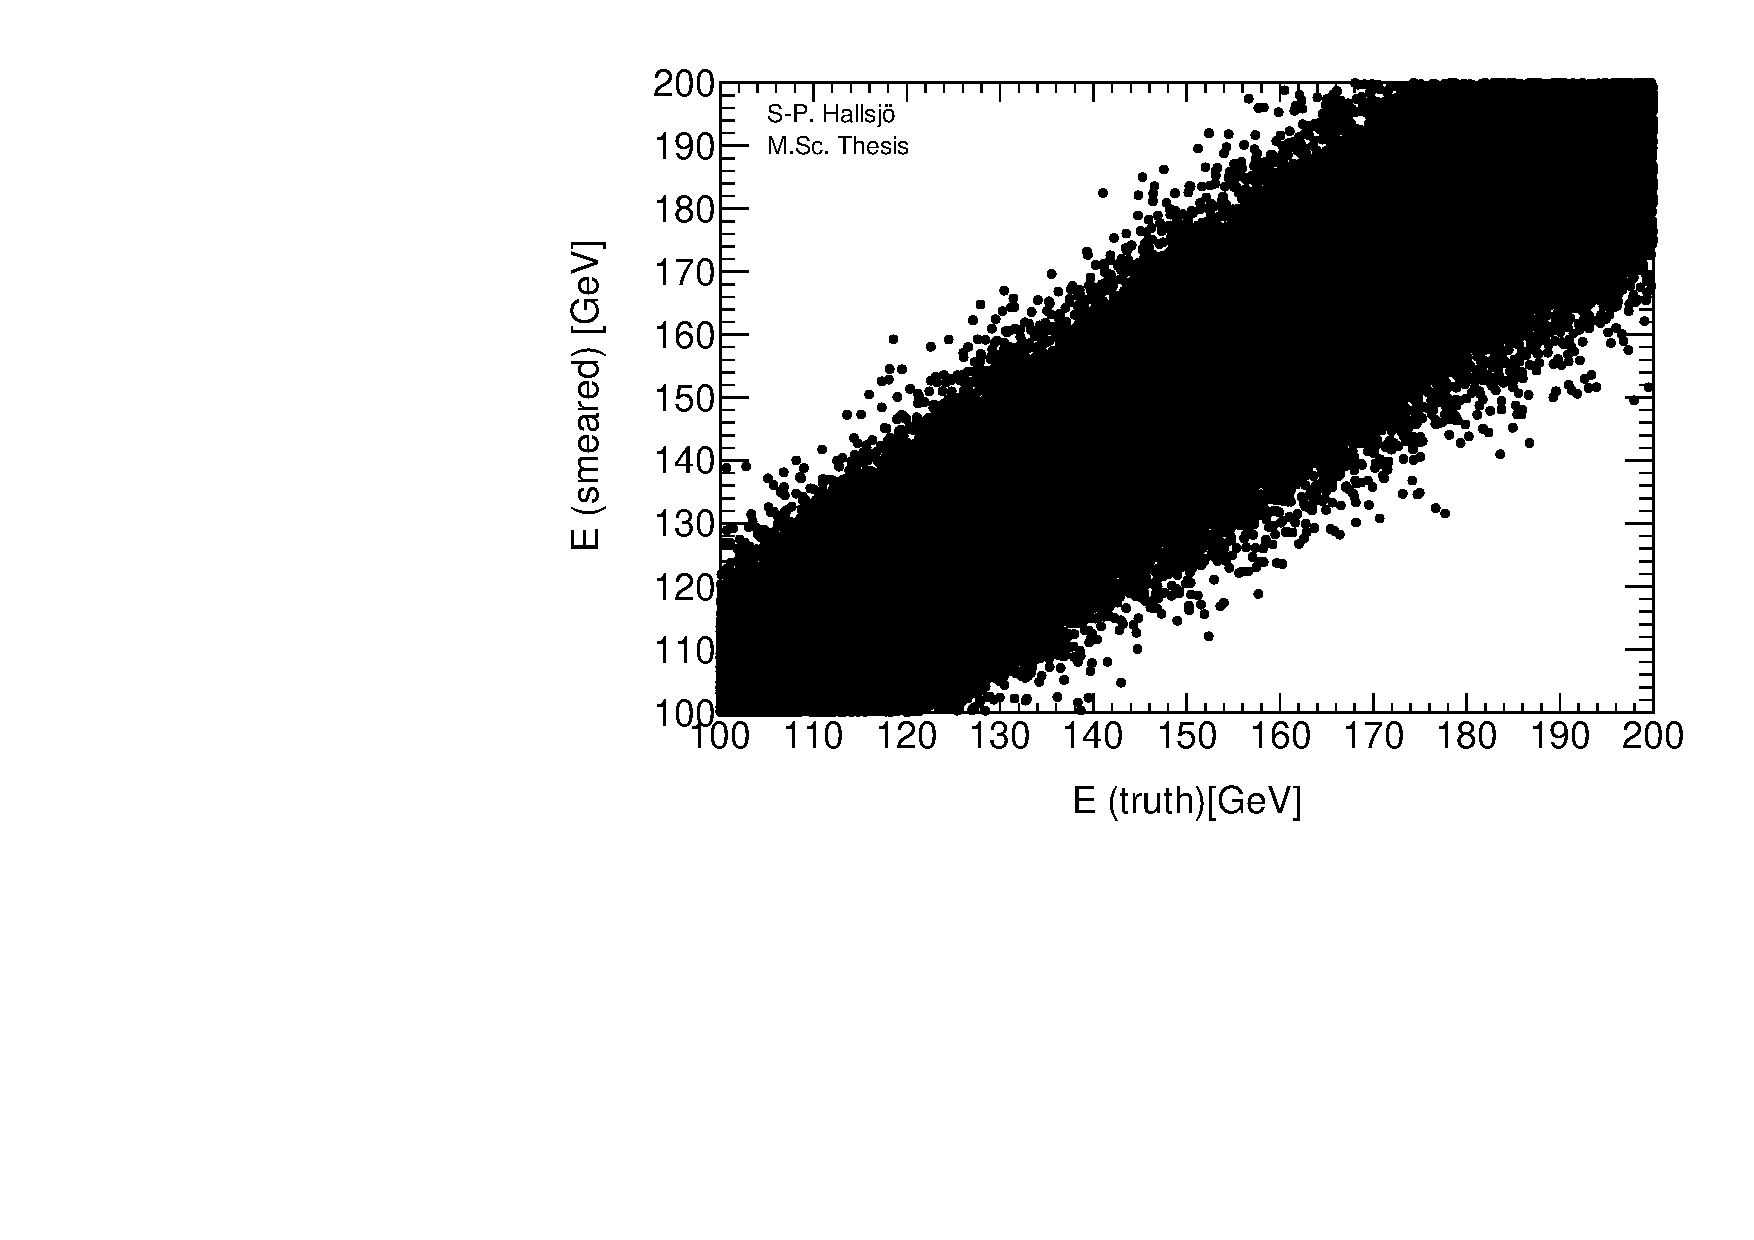
\includegraphics[width=0.5\textwidth]{tau2.pdf}
    }
    \caption{Tau smearing and energy vs smearing plot.}
    \label{fig:tau}
  \end{figure}
  \newpage
\subsection{Jets}
Jets as described in \subsectionref{sec:eo:subsec:mjet}, are hadronic showers. The smearing functions are divided into four different regions depending on the angle $\eta$. 
 \begin{figure}[H] %!ht
    \subfloat[Jet smearing for $\abs{\eta}<0.8$. \label{fig:jet:1}]{%
     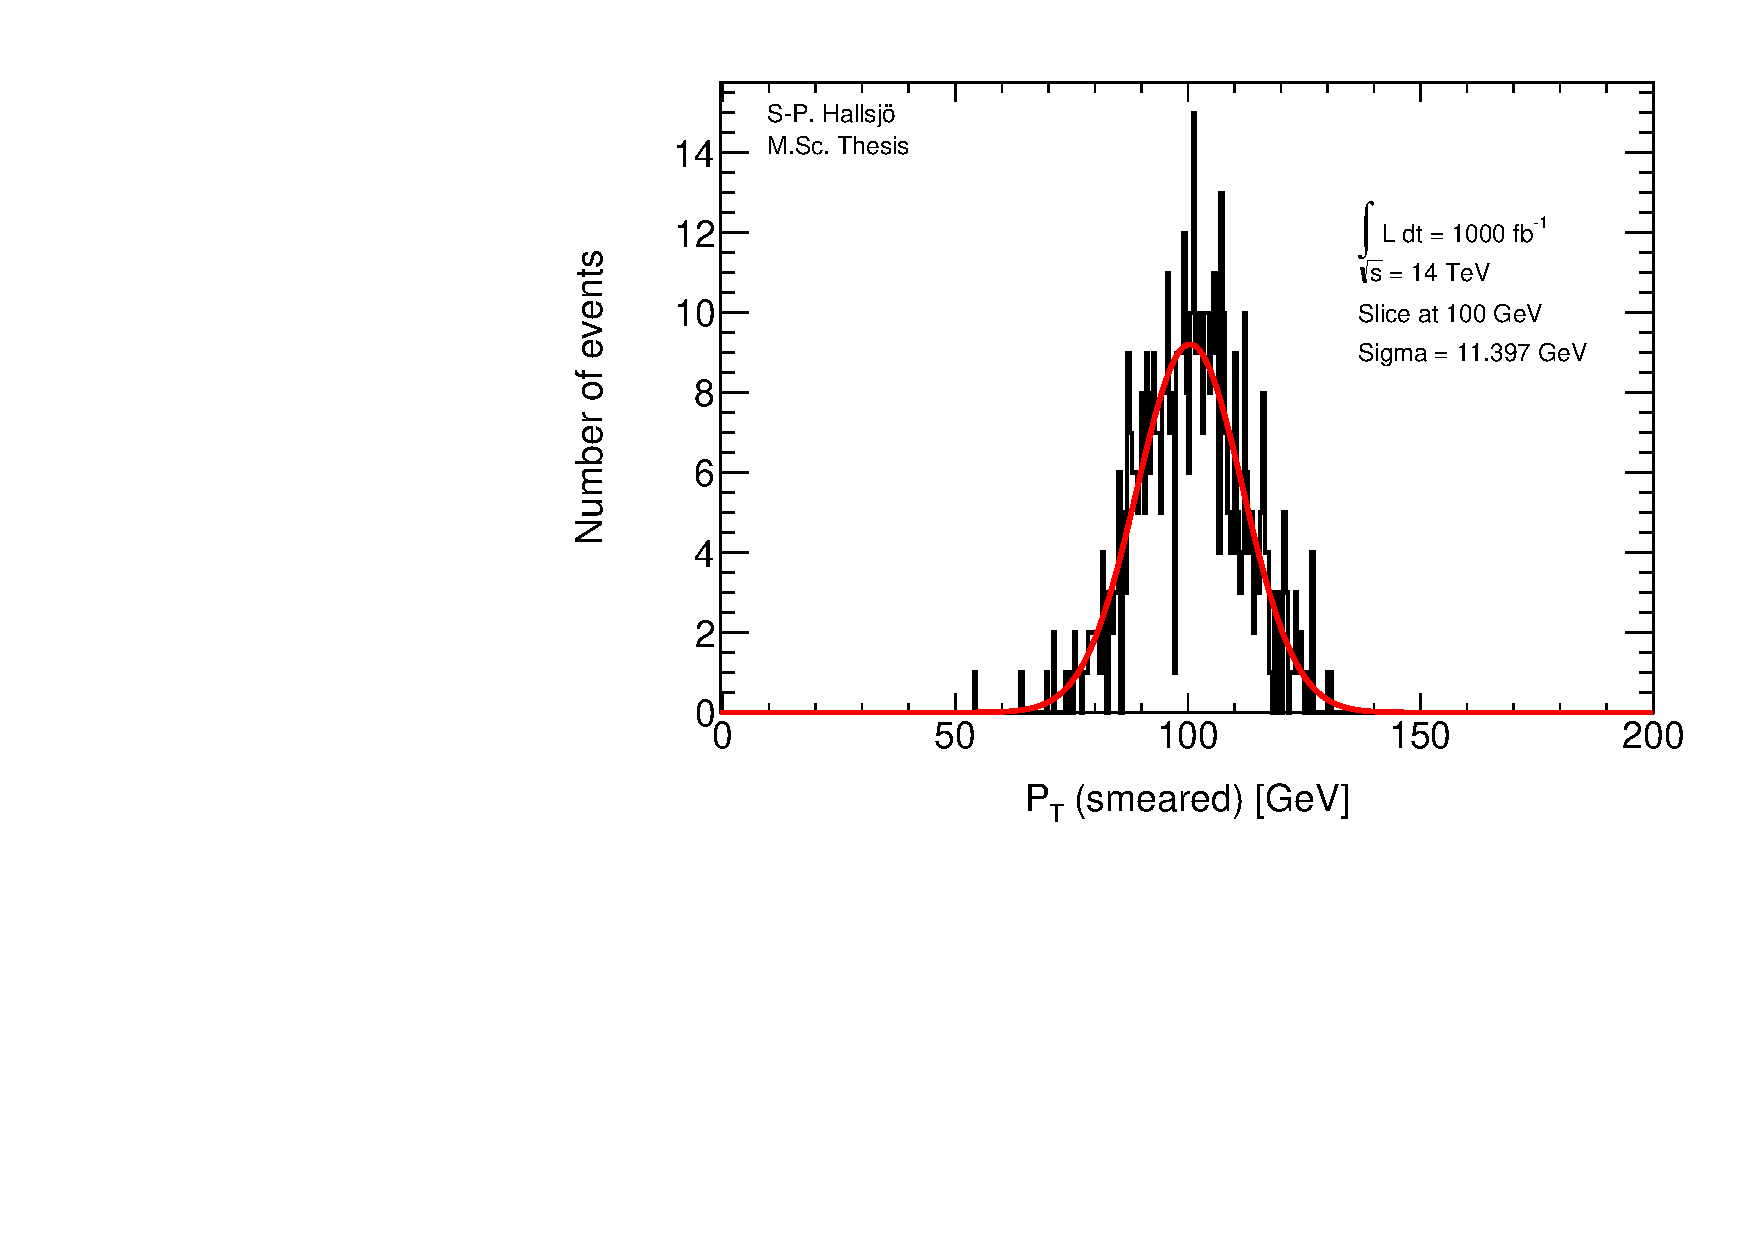
\includegraphics[width=0.5\textwidth]{jeteta1.pdf}
    }
    \hfill
\subfloat[Jet smearing for $0.8<\abs{\eta}<1.2$.\label{fig:jet:2}]{%
      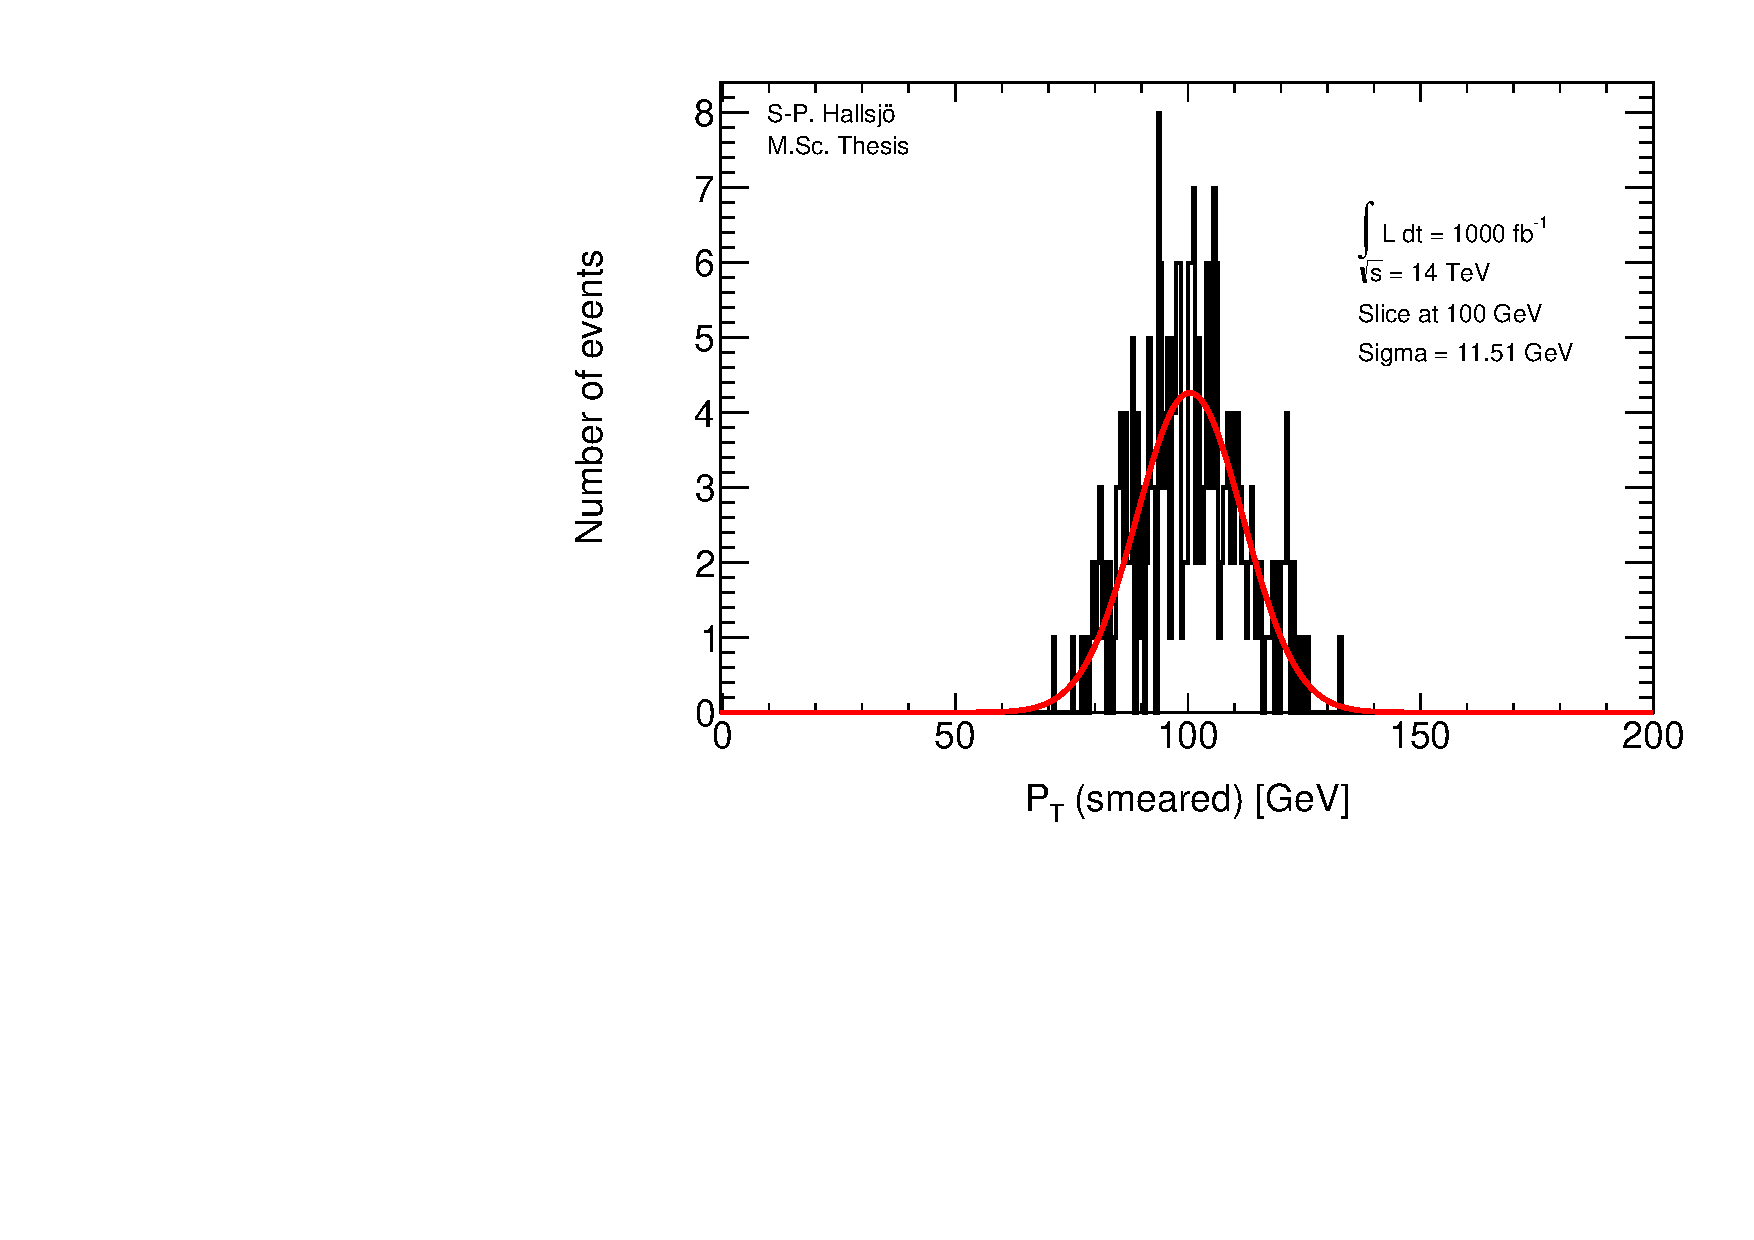
\includegraphics[width=0.5\textwidth]{jeteta2.pdf}
    }
    \hfill
        \subfloat[Jet smearing for $1.2<\abs{\eta}<2.8$. \label{fig:jet:3}]{%
     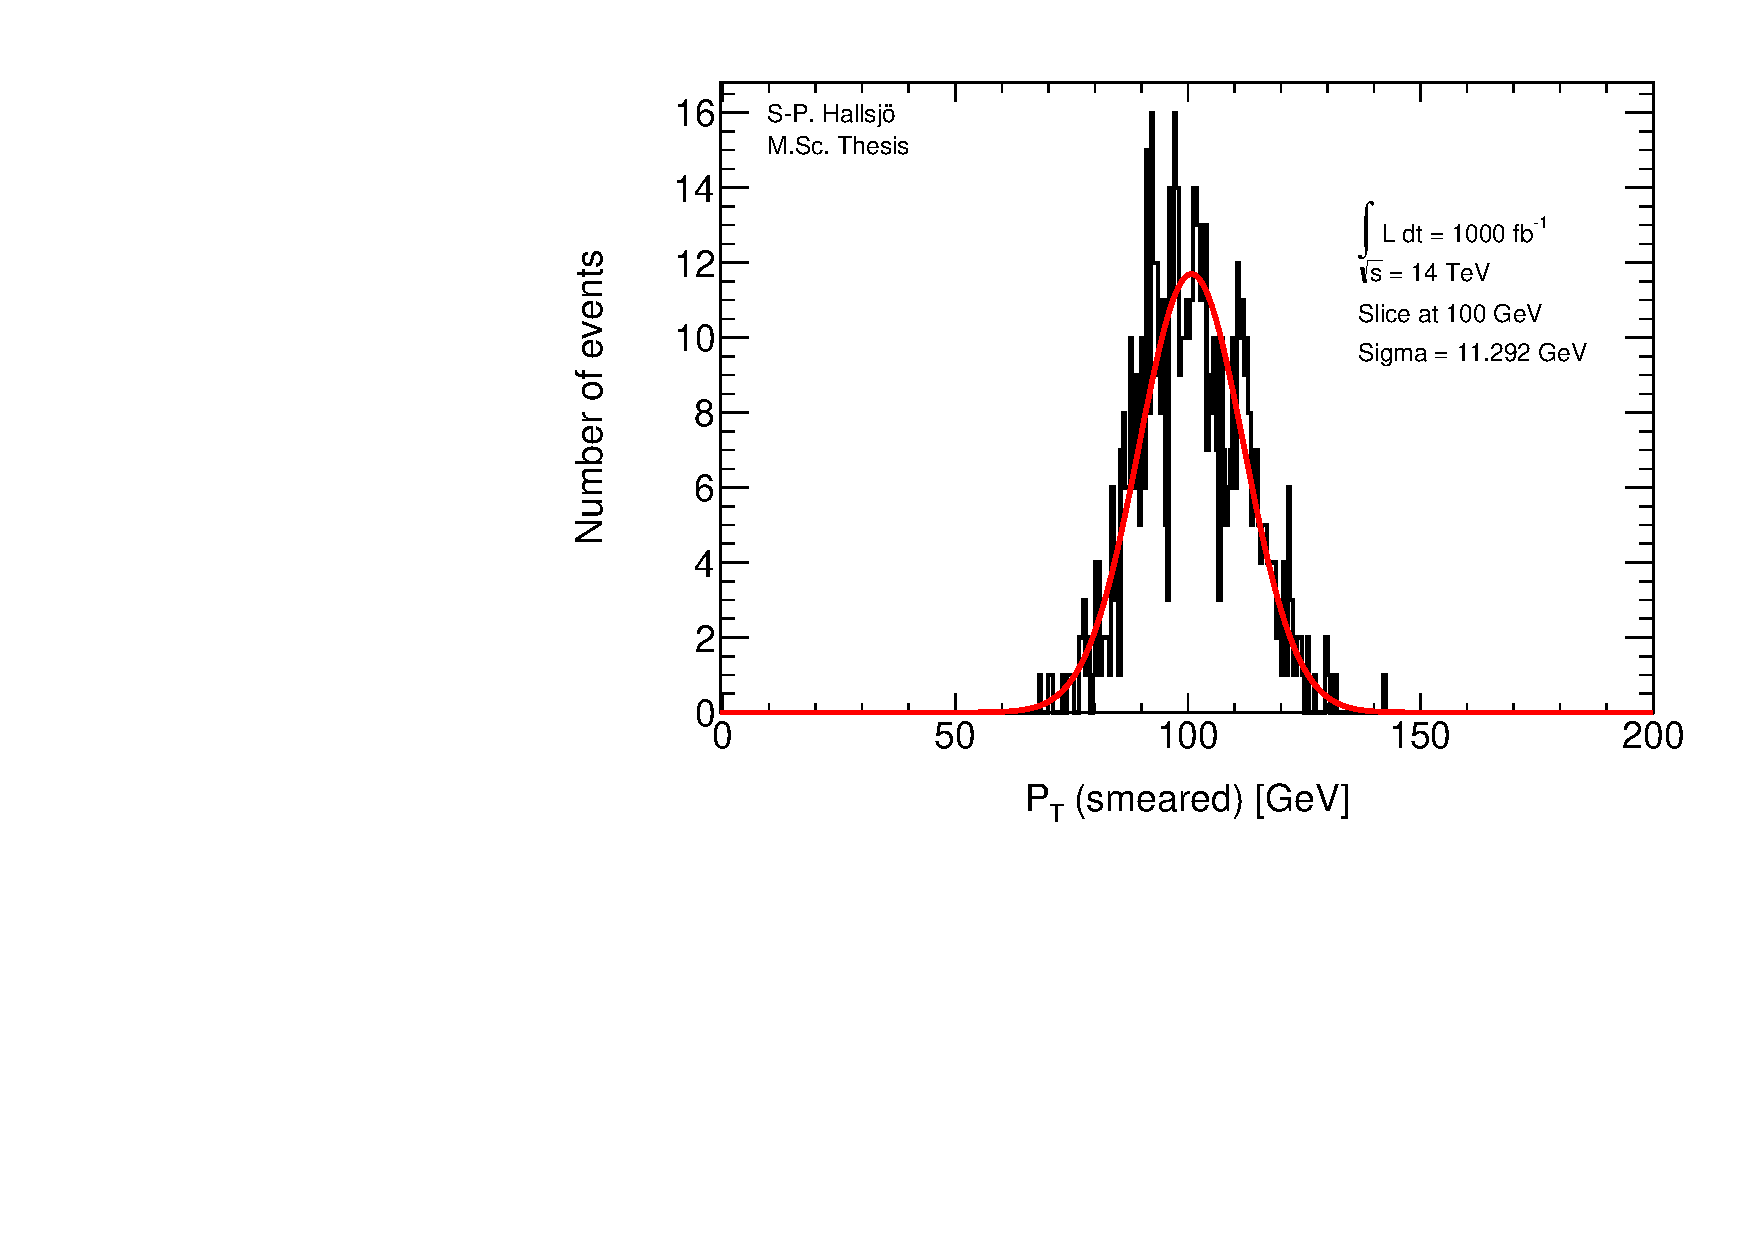
\includegraphics[width=0.5\textwidth]{jeteta3.pdf}
    }
    \hfill
\subfloat[Jet smearing for $2.8<\abs{\eta}<3.6$. \newline Very odd due to the low amount of available data. \label{fig:jet:4}]{%
      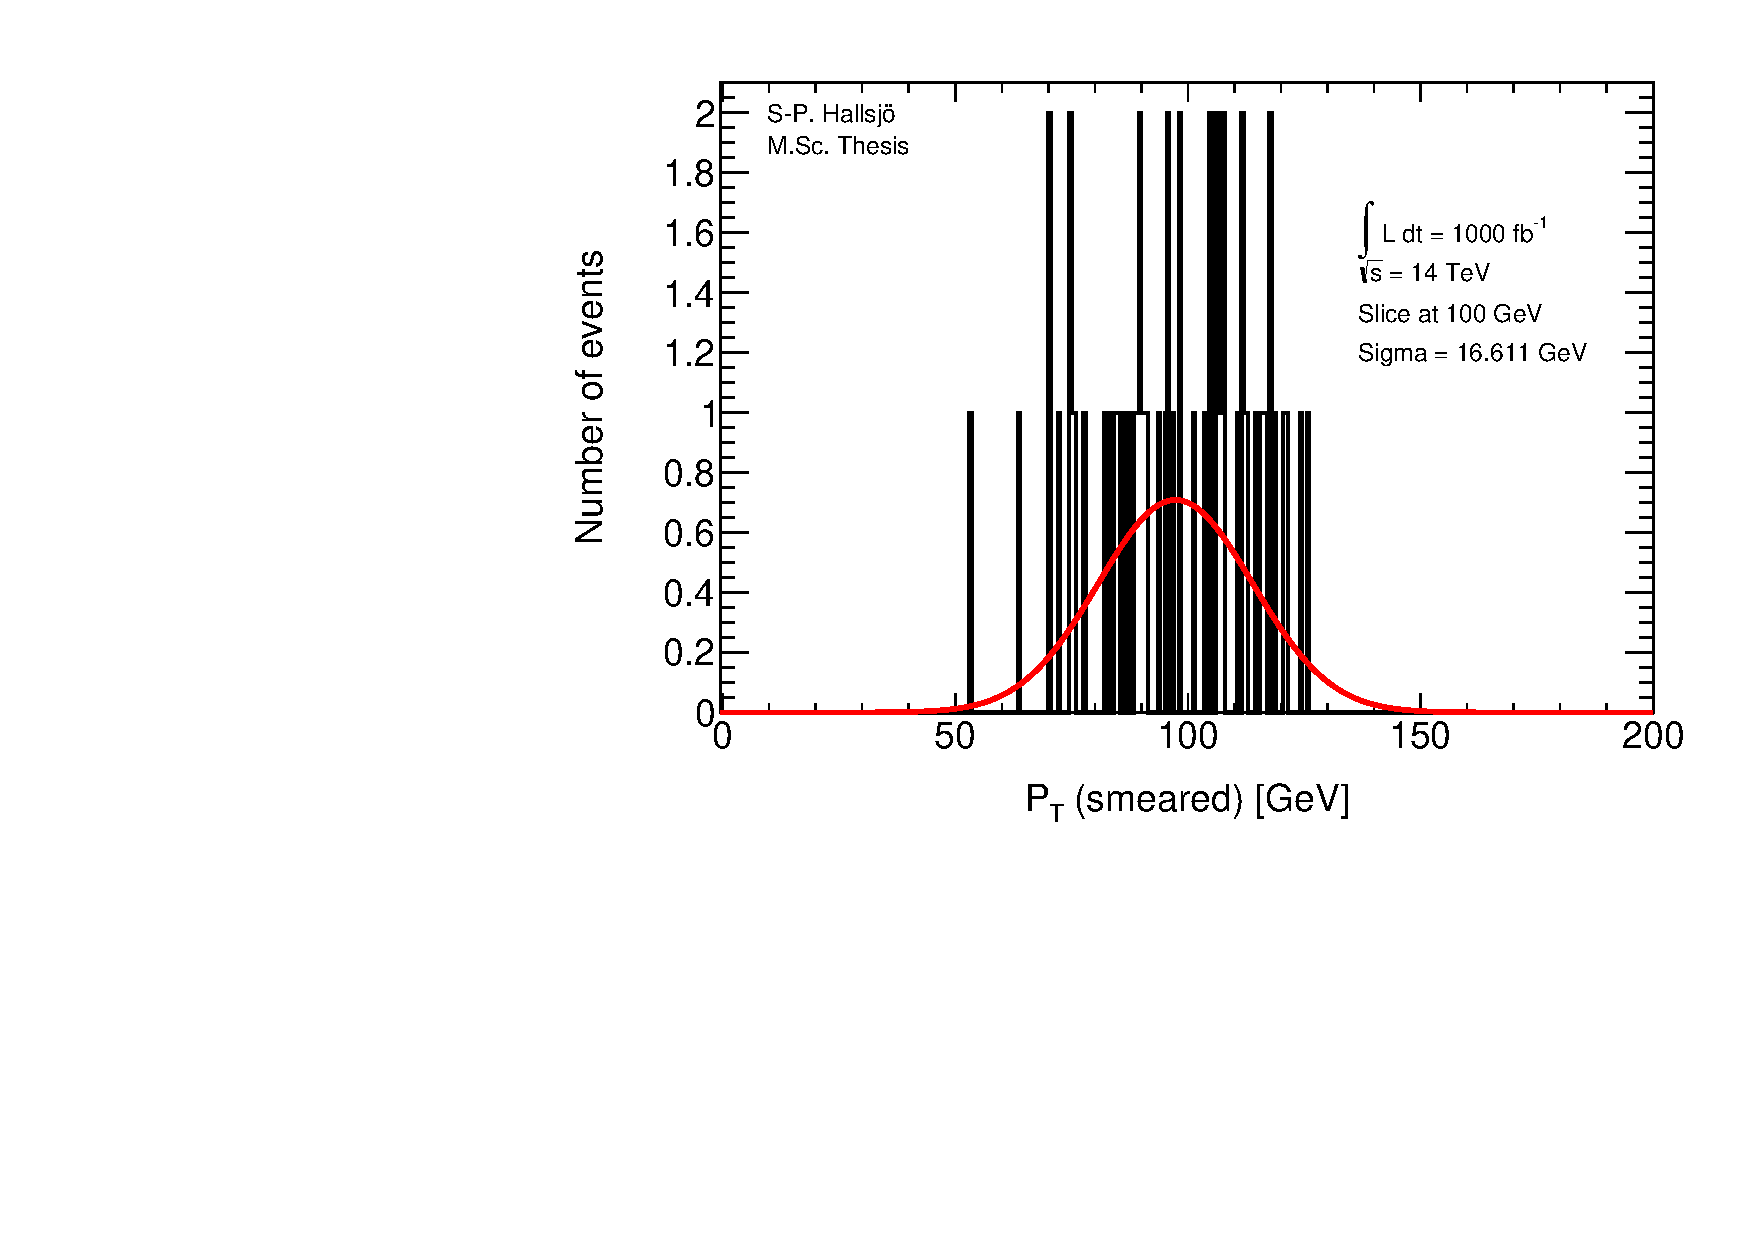
\includegraphics[width=0.5\textwidth]{jeteta4.pdf}
    }
        \hfill
\subfloat[Jet smearing for $\abs{\eta}<0.8$ at $\obs{\mu}=140$. \label{fig:jet:5}]{%
      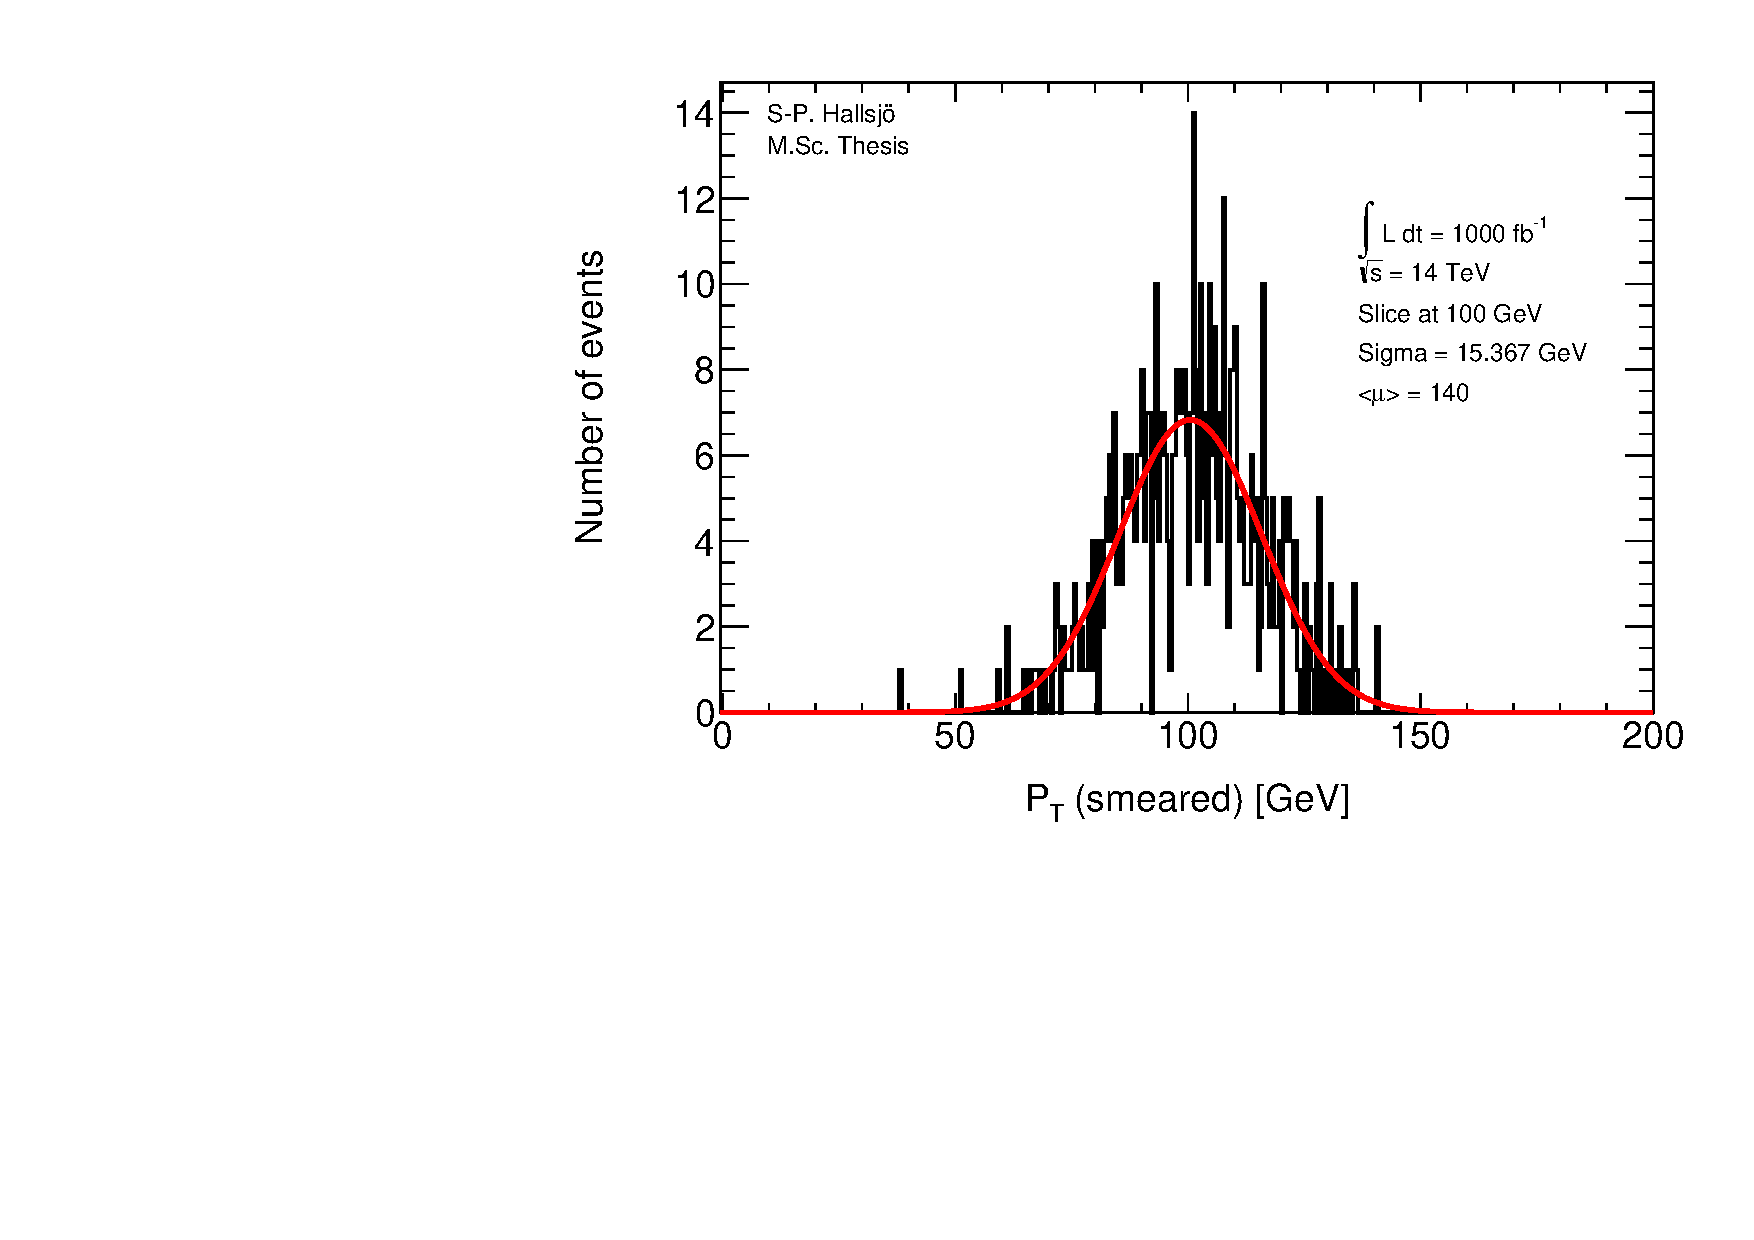
\includegraphics[width=0.5\textwidth]{jeteta1140.pdf}
    }
            \hfill
\subfloat[Jet smearing for $0.8<\abs{\eta}<1.2$ \newline at $\obs{\mu}=140$. \label{fig:jet:6}]{%
      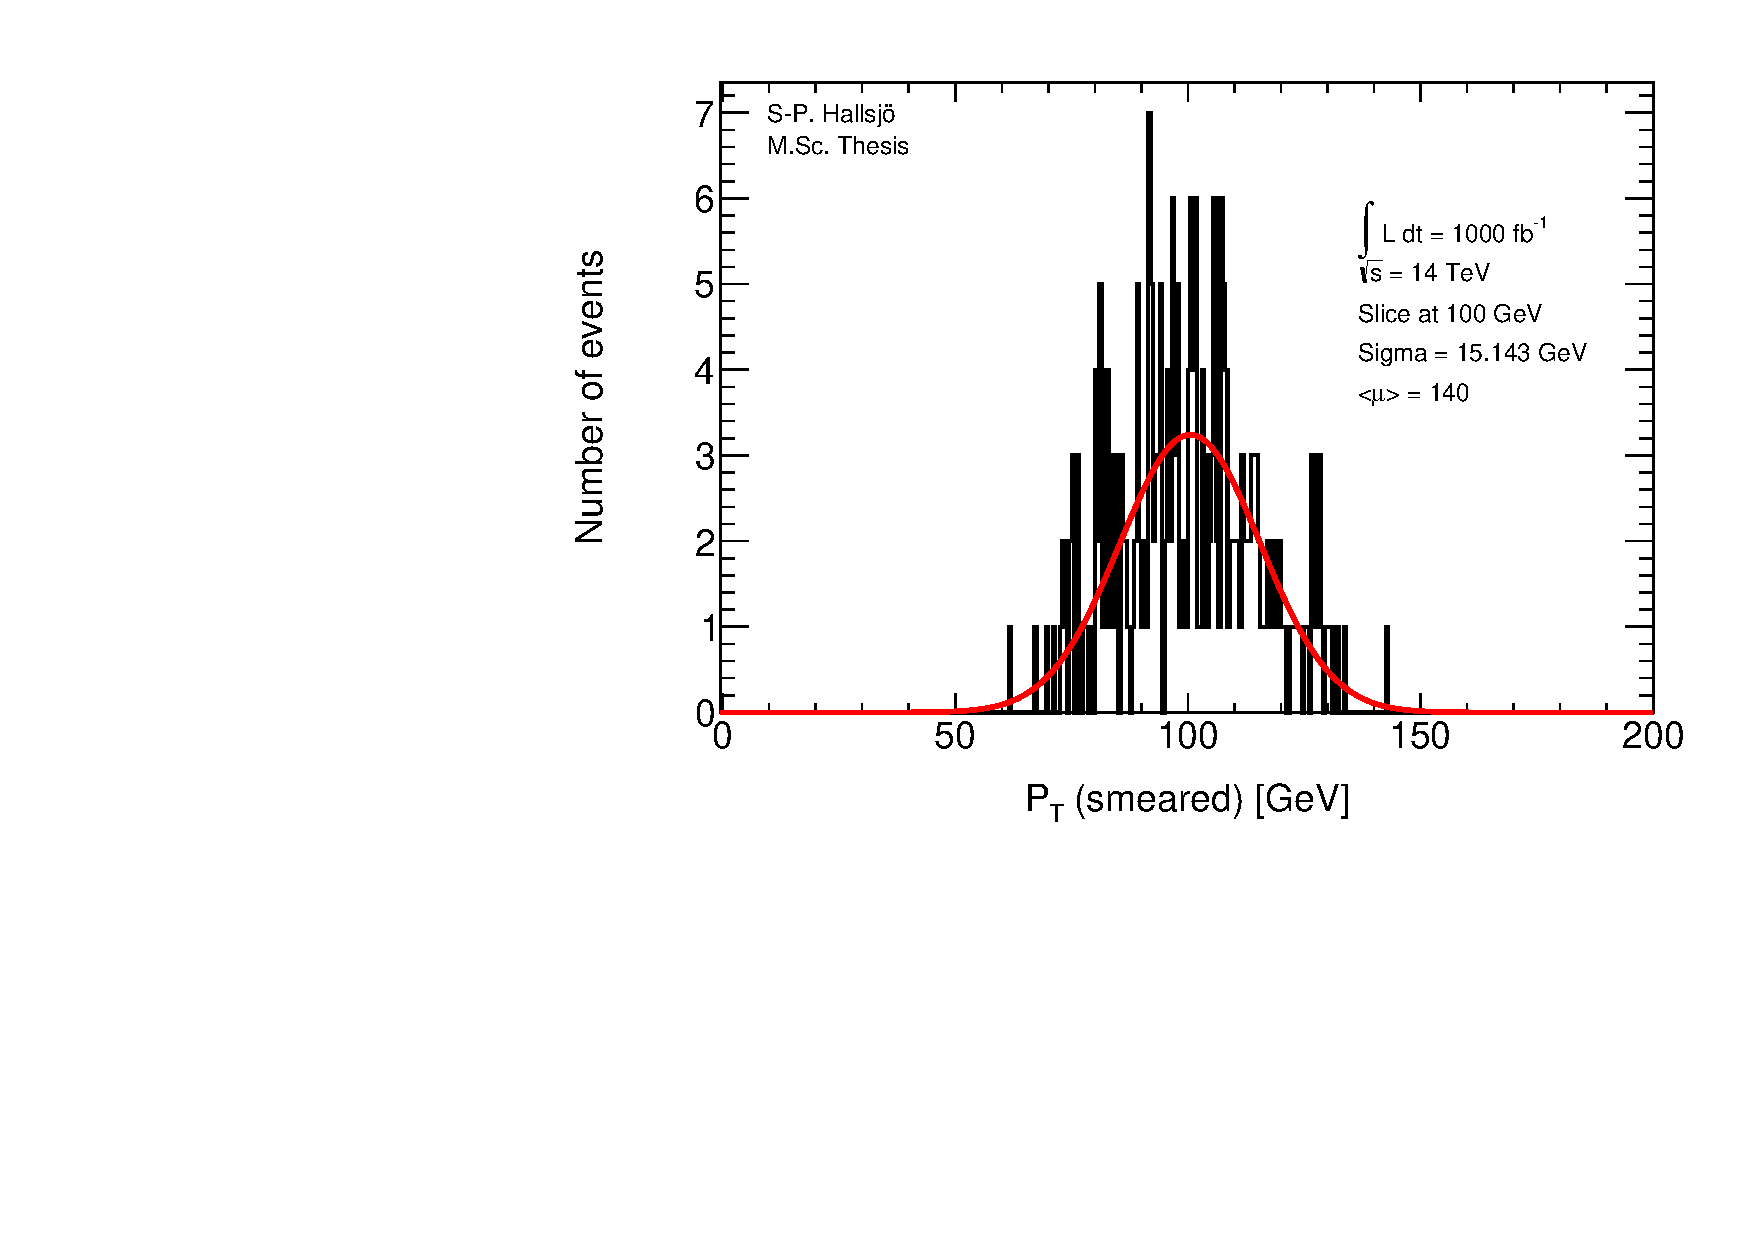
\includegraphics[width=0.5\textwidth]{jeteta2140.pdf}
    }
    \caption{Jet smearing plots.}
    \label{fig:jet}
\end{figure}

\newpage
\subsection{Missing Transversal Energy}
These figures are given as smeared value from origin, thus at 0 it represents that the energy is unsmeared, compared to the others where the slice value represents the unsmeared.

Here the $E_T^{Miss}$ is projected down to the x- and y-axis, since these are the transversal axes, to be smeared. 
 \begin{figure}[H] %!ht
    \subfloat[$E_T^{Miss}$ smearing along the x-axis. \label{fig:MET:x}]{%
     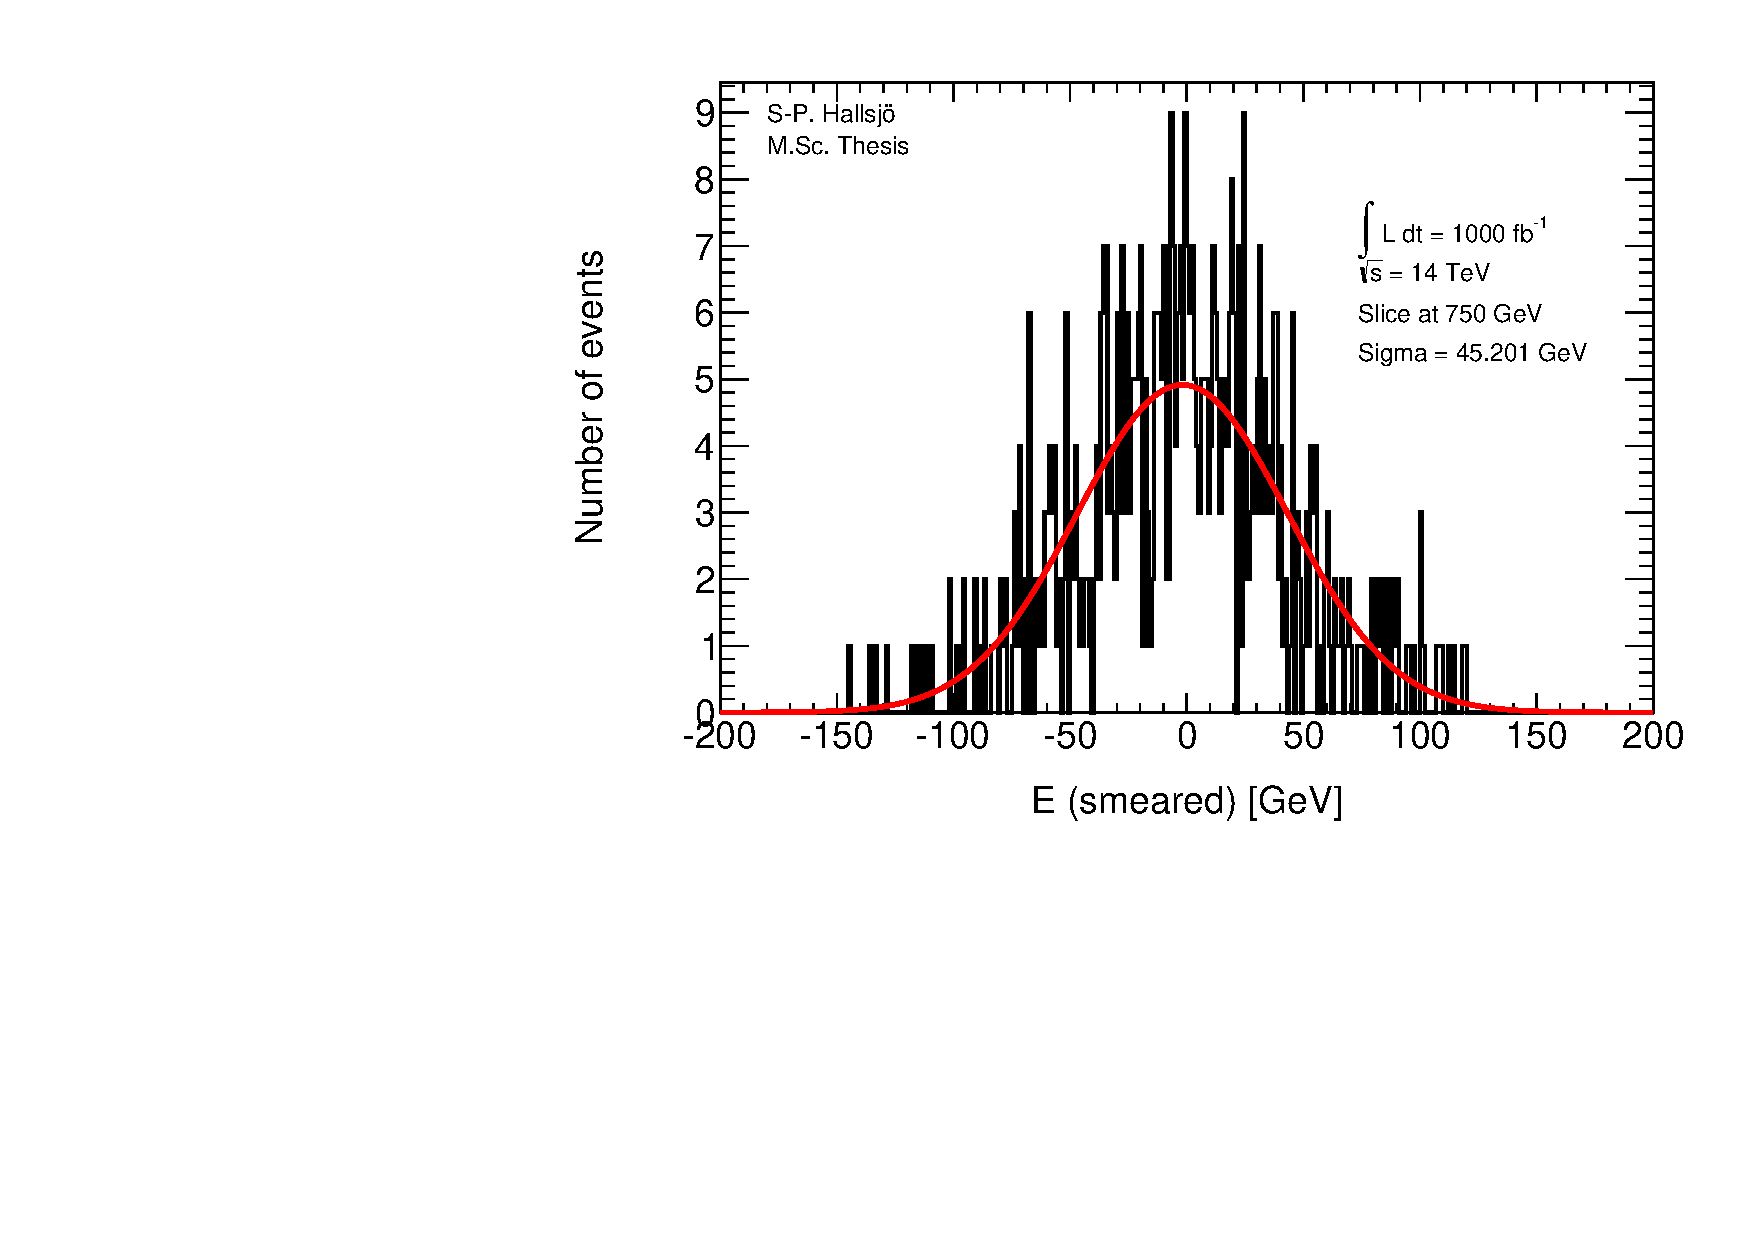
\includegraphics[width=0.5\textwidth]{METx.pdf}
    }
    \hfill
    \subfloat[$E_T^{Miss}$ smearing along the y-axis.\label{fig:MET:y}]{%
      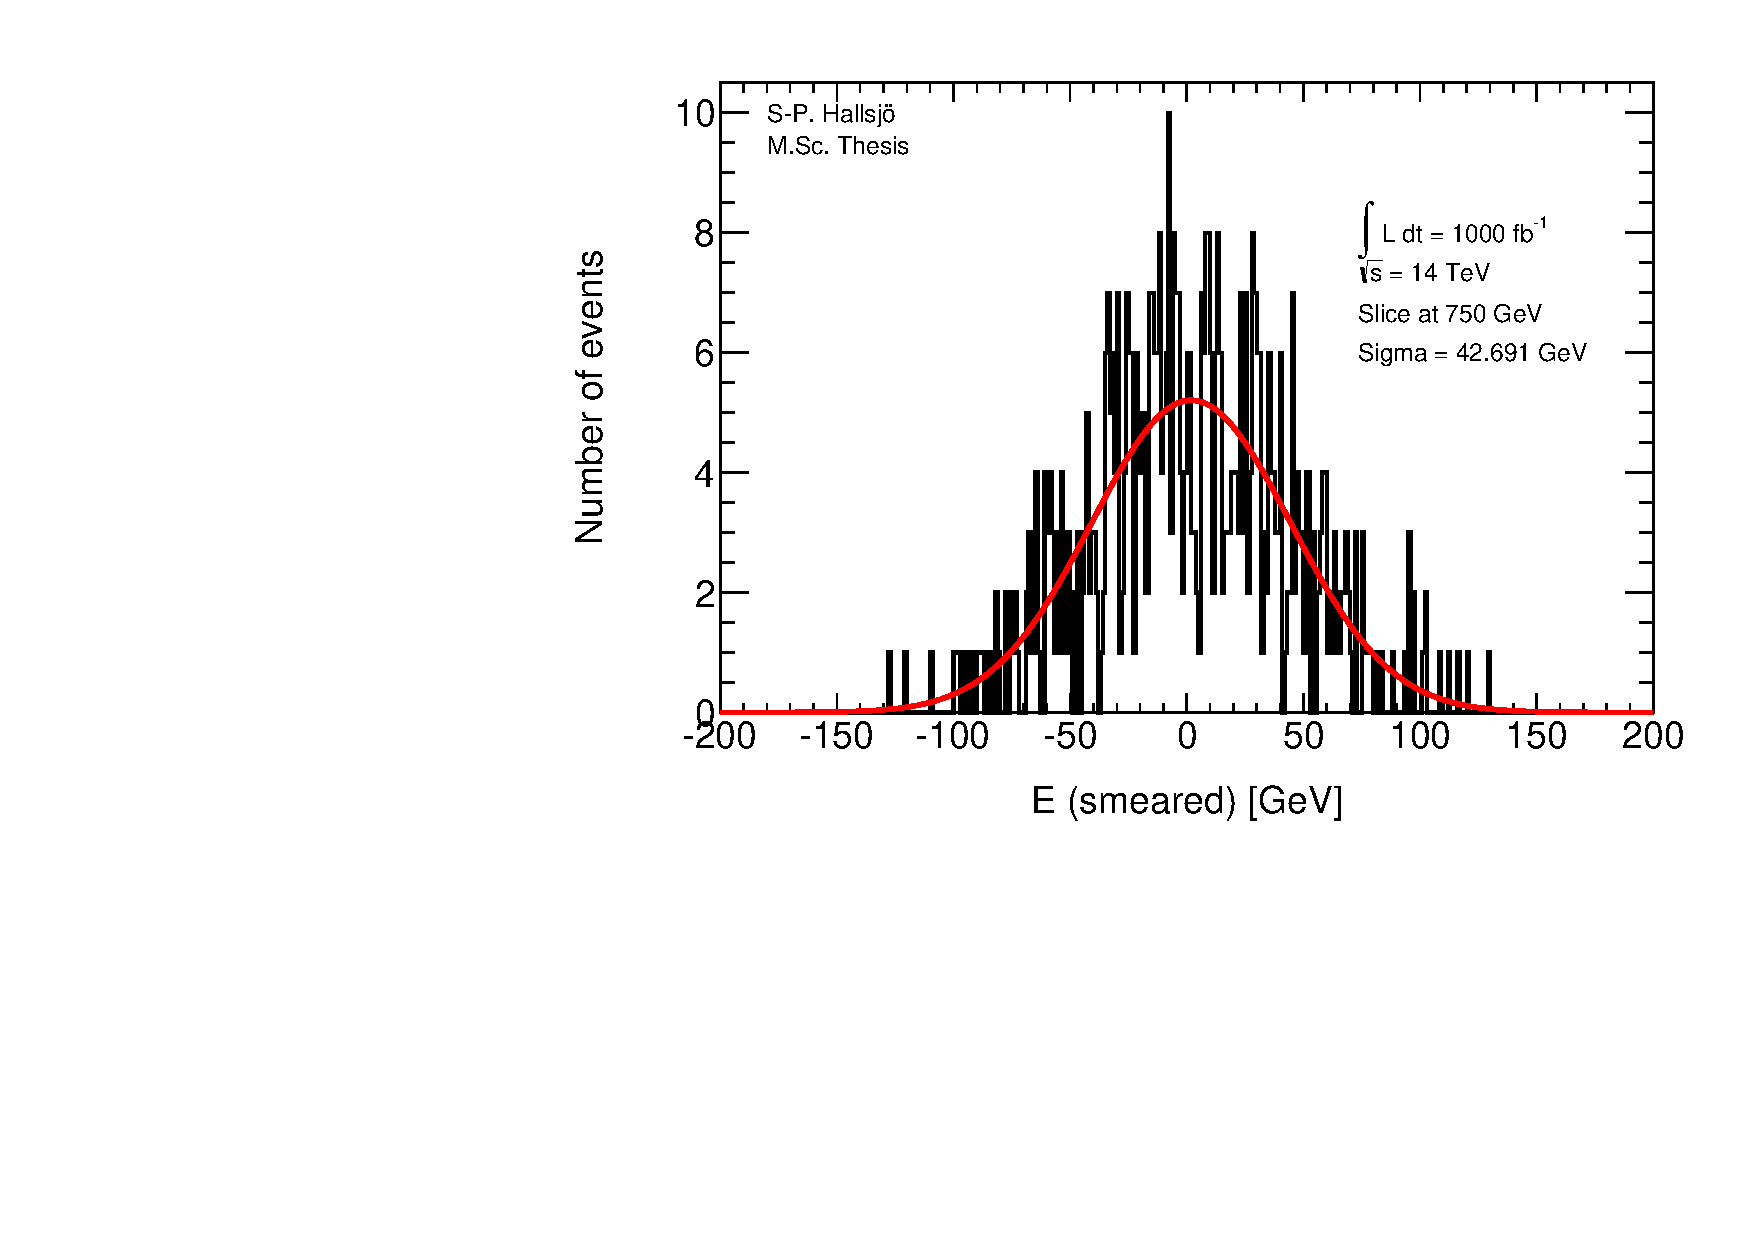
\includegraphics[width=0.5\textwidth]{METy.pdf}
    }
        \hfill
    \subfloat[$E_T^{Miss}$ smearing along the y-axis for $\obs{\mu}=140$.\label{fig:MET:140}]{%
      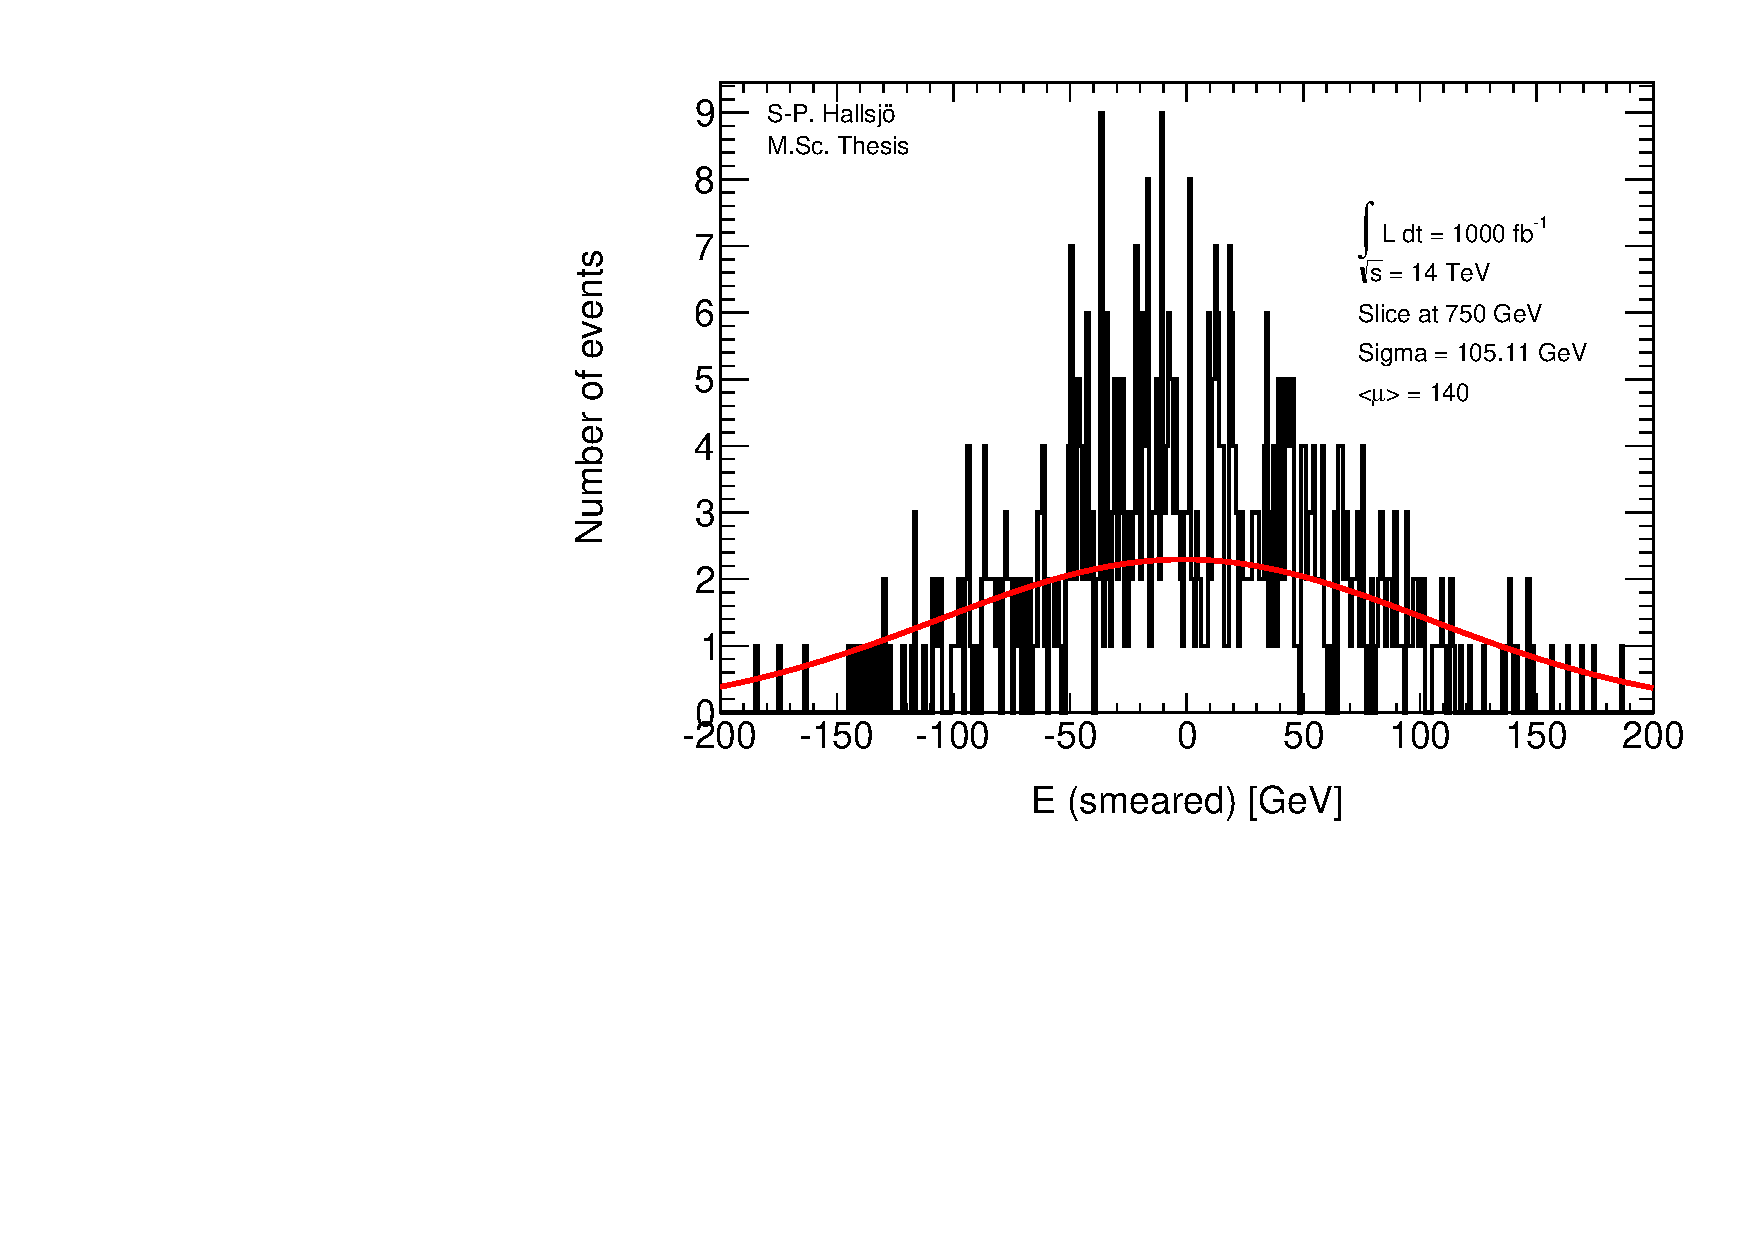
\includegraphics[width=0.5\textwidth]{mety140.pdf}
    }
   \caption{$E_T^{Miss}$ smearing plots}
    \label{fig:MET}
  \end{figure}
\newpage
\section{Expected results}\label{cha:vali:sec:expr}

The expected response has been calculated and taken from \citep{ATL-PHYS-PUB-2013-004}.

The independence of pile-up for leptons and photons is backed up in previous research, for instance \citep{Electronperf:2011, ATLAS:LOI2} were the first states:
\begin{quotation}
``The uncertainty due to pile-up was investigated by comparing simulated MC samples with and without pile-up and was found to be negligible''
\end{quotation}
This is also confirmed in other internal documents.


To validate the smearing code comparisons were made with \citep{ATL-PHYS-PUB-2013-004} which gave the following formulation for the expected \abbrRMS: 
\begin{table}[H]
\renewcommand{\arraystretch}{1.5} %Change height of tabel
\begin{center}
\begin{tabular}{|l|l|}
\hline
Process & Absolute \abbrRMS \\ \hline
Electron \& photon & $\sigma=0.3\oplus 0.1\sqrt{E(GeV)}\oplus 0.01E(GeV)$, $|\eta|<$ 1.4 \\
& $\sigma=0.3\oplus 0.15\sqrt{E(GeV)}\oplus 0.015E(GeV)$, 1.4 $<|\eta|<$ 2.47 \\ \hline 
Muon & $\sigma=\frac{\sigma_{id} \sigma_{ms}}{\sigma_{id} \oplus \sigma_{ms}}$\\
& $\sigma_{id}=P_T(a_1 \oplus a_2 P_T)$\\
& $\sigma_{ms}=P_T(\frac{b_0}{P_T} \oplus b_1 \oplus b_2 P_T)$\\ \hline
Tau & $\sigma =(0.03\oplus \frac{0.76}{\sqrt{E(GeV)}})E(GeV)$ \\ \hline
Jet & $\sigma = P_T(GeV)(\frac{N}{P_T} \oplus \frac{S}{\sqrt{P_T}} \oplus C)$ \\ \hline
$E_T^{Miss}$ & $\sigma = (0.4+0.09\sqrt{\mu})\sqrt{\sum E(GeV)+20\mu}$ \\ \hline
\end{tabular}
\end{center}
\renewcommand{\arraystretch}{1.0} %Change back
\caption{Expected absolute \abbrRMS.}
\label{tab:expected RMS}
\end{table}
\begin{itemize}
%\item For muon: Where a$_i$ and b$_i$ are dependent on $\eta$.
\item For muon: All parameters are given in \tableref{tab:muonparam}.
\item For tau: Fixed at 3 prong. 1 prong exists though was not used in this thesis. \\
Where prong refers to the different amount of tracks that from which they were reconstructed.
%\item For Jet: Where N, S, and C depend on $\eta$. N is also dependent on the pile-up that is simulated.\\
\item For jet: All parameters are given in \tableref{tab:jetparam} where $N=a(\eta)+b(\eta)\mu$.
%Where $\eta$ is the same as discussed in \subsectionref{sec:eo:subsec:coord}
%\item All parameters can be found in \citep{ATL-PHYS-PUB-2013-004}.
\end{itemize}

\begin{table}[H]
\renewcommand{\arraystretch}{1.5} %Change height of tabel
\begin{center}
\begin{tabular}{|l|l|l|l|l|l|}
\hline
 &$a_1$&$a_2$&$b_0$&$b_1$&$b_2$ \\ \hline
$\abs{\eta}<1.05$&0.01607&0.000307&0.24&0.02676&0.00012 \\ \hline
$\abs{\eta}<1.05$&0.03000&03000387&0.00&0.03880&0.00016 \\ \hline
\end{tabular}
\end{center}
\caption{Parameters used in the muon smearing function take from \citep{ATL-PHYS-PUB-2013-004}.}
\label{tab:muonparam}
\renewcommand{\arraystretch}{1.0} %Change back
\end{table}
\begin{table}[H]
\renewcommand{\arraystretch}{1.5} %Change height of tabel
\begin{center}
\begin{tabular}{|l|l|l|l|l|}
\hline
$\abs{\eta}$&a&b&S&C \\ \hline
0-0.8&3.2&0.07&0.74&0.05 \\
0.8-1.2&3.0&0.07&0.81&0.05 \\
1.2-2.8&3.3&0.08&0.54&0.05 \\
2.8-3.6&2.8&0.11&0.83&0.05 \\ \hline
\end{tabular}
\end{center}
\caption{Parameters used in the jet smearing function taken from \citep{ATL-PHYS-PUB-2013-004}.}
\label{tab:jetparam}
\renewcommand{\arraystretch}{1.0} %Change back
\end{table}

\begin{table}[H]
\begin{center}
\begin{tabular}{|l|l|l|l|l|}
\hline
Process&\abbrRMS [GeV]&Error in \abbrRMS &Expected \abbrRMS & Significance\\ \hline
Electron low $\eta$&1.24948&0.0481987&1.18427&1.35286\\
High $\eta$&1.8211&0.141329&1.74446&0.542334\\ \hline
Photon low $\eta$&1.18986&0.0400187&1.18427&0.139734\\
High $\eta$&1.80297&0.0374312&1.74446&1.56323\\ \hline
Muon low $\eta$&1.19016&0.0524938&1.49789&5.86235\\
High $\eta$&1.70694&0.0882606&2.18318&5.39575\\ \hline
Tau&10.8992&0.299761&10.3388&1.86975\\ \hline
Jet low $\eta$&11.3974&0.351391&11.5983&0.571586\\
$\obs{\mu}=140$&15.3673&0.473783&15.7721&0.854499\\
Mid low $\eta$&11.5096&0.518872&11.9352&0.820407\\
$\obs{\mu}=140$&15.1427&0.682649&15.9515&1.18475\\
Mid high $\eta$&11.2916&0.310314&10.9439&1.12021\\
High $\eta$&16.6112&1.52891&13.5&2.03491\\ \hline
$E_T^{Miss} $x$-$axis&45.2013&1.35426&48.4483&2.39762\\ \hline
$E_T^{Miss} $y$-$axis&42.6906&2.27904&48.4483&4.50154\\ 
$\obs{\mu}=140$&105.109&12.239&87.2812&1.45667\\  \hline
\end{tabular}
\end{center}
\caption{\abbrRMS values.}
\label{tab:RMSval}
\end{table}
\begin{itemize}
\item Where the given \abbrRMS is still the absolute. 
\item The significance is the standard deviation of between the expected and calculated with respect to the error.
\end{itemize}
\newpage
\section{Discussion}
\subsection{Smearing independent on pile-up}
From the validation done it was interesting to note that the smearing functions were created from previous studies, \citep{Electronperf:2011, ATLAS:LOI2}, which had shown that leptons and photons are not affected by pile-up.
This may seem incredible however it becomes quite logical when one understands how the detectors work. To be able to detect particles the detectors must detect an excess of energy which comes from a particle passing through. This should not be distorted by an increased pile-up. The amount of particles passing through will of course increase, but the detections should be unaffected as well as the recreation of the events. However with the same logic it makes sense that jets and $E_T^{Miss}$ are quite affected since they are combined of several parts, either hadronic particles or by all the transversal missing energy. 

Another interesting part is how the effect diminishes with and increasing energy. As seen above, and through the the formula, for the high energies which were of interest here the effect is minimal. 
\subsection{Comparison to expected results}
One of the major problems in the comparison was to get the significance of the Gaussian fit to be calculated correctly. The tool ROOT has a lot of different features which made this task somewhat difficult. Also since this is a statistical property there is a statistical fluctuation in the result. 

Another was to retrieve the correct values from the paper, \citep{ATL-PHYS-PUB-2013-004}, since it was unclear if the values given were absolute or scale dependent. This has now been corrected in a new version of the paper.
\newpage
\section{Conclusion}
The smearing functions work as intended within 5.8 sigma, however when using a test box and averaging the sigmas one ends up with half of this for the extreme cases, muons and $E_T^{Miss} $y$-$axis.